% 导言区
\documentclass[a4paper,]{article}

% 导入中文宏
\usepackage{ctex}
\usepackage{underscore}
\usepackage{array}
\usepackage{setspace}
\usepackage{enumerate}
\usepackage[margin=1in]{geometry}
\usepackage{titlesec,titletoc}
\usepackage[titles]{tocloft}
\usepackage{tocloft}
\usepackage{booktabs}
\usepackage{graphicx}
\usepackage{amsmath}
\usepackage{cite}
\usepackage{appendix}
\usepackage{listings}
\usepackage{xcolor}
\usepackage{fontspec}
\usepackage{setspace}
\usepackage{algorithm}  
\usepackage{algpseudocode}
\usepackage{amssymb}
\usepackage{subfigure}

% 构建命令,取别名,使用degree 代替 ^ circ
\renewcommand{\algorithmicrequire}{\textbf{输入}}  % Use Input in the format of Algorithm  
\renewcommand{\algorithmicensure}{\textbf{输出}} % Use Output in the format of Algorithm
\floatname{algorithm}{算法} 
\newcommand\degree{^\circ}
\newcommand{\chuhao}{\fontsize{42pt}{\baselineskip}\selectfont}
\newcommand{\xiaochuhao}{\fontsize{36pt}{\baselineskip}\selectfont}
\newcommand{\yihao}{\fontsize{28pt}{\baselineskip}\selectfont}
\newcommand{\erhao}{\fontsize{21pt}{\baselineskip}\selectfont}
\newcommand{\xiaoerhao}{\fontsize{18pt}{\baselineskip}\selectfont}
\newcommand{\sanhao}{\fontsize{15.75pt}{\baselineskip}\selectfont}
\newcommand{\sihao}{\fontsize{14pt}{\baselineskip}\selectfont}
\newcommand{\xiaosihao}{\fontsize{12pt}{\baselineskip}\selectfont}
\newcommand{\wuhao}{\fontsize{10.5pt}{\baselineskip}\selectfont}
\newcommand{\xiaowuhao}{\fontsize{9pt}{\baselineskip}\selectfont}
\newcommand{\liuhao}{\fontsize{7.875pt}{\baselineskip}\selectfont}
\newcommand{\qihao}{\fontsize{5.25pt}{\baselineskip}\selectfont}
\newcommand{\zw}{\setlength{\baselineskip}{1.5em}\xiaosihao}
\newcommand\listexamplename{目录}
\newtheorem{Proof}{证明}
\renewcommand\arraystretch{1.5}
\usepackage[titles]{tocloft}
\renewcommand{\cftsecleader}{\cftdotfill{\cftdotsep}}

\makeatletter
\renewcommand{\numberline}[1]{%
	\settowidth\@tempdimb{#1\hspace{0.5em}}%
	\ifdim\@tempdima<\@tempdimb%
	\@tempdima=\@tempdimb%
	\fi%
	\hb@xt@\@tempdima{\@cftbsnum #1\@cftasnum\hfil}\@cftasnumb}
\makeatother
	\lstset{ %
	language=Python,                % the language of the code
	%numbers=left,                   % where to put the line-numbers
	%numberstyle=\tiny\color{gray},  % the style that is used for the line-numbers
	%numbersep=5pt,                  % how far the line-numbers are from the code
	showspaces=false,               % show spaces adding particular underscores
	showstringspaces=false,         % underline spaces within strings
	showtabs=false,                 % show tabs within strings adding particular underscores
	frame=lines,
	%rulecolor=\color{black},        % if not set, the frame-color may be changed on line-breaks within not-black text (e.g.
	tabsize=4,                      % sets default tabsize to 2 spaces
	captionpos=b,                   % sets the caption-position to bottom
	breaklines=true,                % sets automatic line breaking
	breakatwhitespace=false,        % sets if automatic breaks should only happen at whitespace
	title=\lstname,                 % show the filename of files included with \lstinputlisting;
	% also try caption instead of title
	basicstyle=\small\fontspec{Courier New},
	keywordstyle=\color[RGB]{40,40,255},          % keyword style
	commentstyle=\color{gray},       % comment style
	stringstyle=\rmfamily\slshape\color[RGB]{128,0,0},         % string literal style
	escapeinside={\%*}{*)},            % if you want to add LaTeX within your code
	morekeywords={delete,PLSRegression,fit,predict,tolist,append,error,Sequential,Linear,Sigmoid,cuda,MSELoss,Adam,parameters,read_csv,ones,vstack,dot,solve}               % if you want to add more keywords to the set
}

%从这开始讲解点:1、定义开头
\title{\heiti SparkDebate星火智能辩论平台\\

}
%讲解点2、是否显示日期
\date{2023.9.25}
% 正文区
\begin{document}
		\maketitle
	\thispagestyle{empty}
	\begin{table}[ht]
	\centering
	\renewcommand\arraystretch{4}
	\vskip 3.5cm
	%讲解点3:队员表,不用改
	\begin{tabular}{ccccc}
	\hline
	\sanhao{姓名}&\qquad\qquad&\sanhao{学校}&\qquad\qquad&\sanhao{专业}\\
	\hline
	\sanhao{黄柏特}&\qquad\qquad&\sanhao{西安电子科技大学}&\qquad\qquad&\sanhao{人工智能专业}\\
	\sanhao{潘笃驿}&\qquad\qquad&\sanhao{西安电子科技大学}&\qquad\qquad&\sanhao{人工智能专业}\\
	\sanhao{林伟龙}&\qquad\qquad&\sanhao{西安电子科技大学}&\qquad\qquad&\sanhao{数据科学与大数据技术专业}\\
	\sanhao{王天羿}&\qquad\qquad&\sanhao{西安电子科技大学}&\qquad\qquad&\sanhao{计算机科学与技术专业}\\
	\sanhao{孙一凡}&\qquad\qquad&\sanhao{西安电子科技大学}&\qquad\qquad&\sanhao{网络工程专业}\\
	\sanhao{安敏瑜}&\qquad\qquad&\sanhao{西安电子科技大学}&\qquad\qquad&\sanhao{信息工程专业}\\
	\sanhao{邓佳}&\qquad\qquad&\sanhao{西安邮电大学}&\qquad\qquad&\sanhao{机器人工程专业}\\
	\hline
\end{tabular}
\end{table}
	
	\newpage
	
	%讲解点4、论文标题 + 摘要 + 关键词 设置
	\begin{center}
	
		\xiaoerhao{\heiti 基于星火大模型开发的智能辩论平台}
		
		\vskip 0.5cm
		
		\sanhao{\heiti 项目简介}\\
		
	\end{center}
	
	\zw{
		SparkDebate是基于星火大模型的智能辩论平台。通过星火大模型,星火助手API,前端Vue框架,提示词工程与Langchain技术实现了优秀的辩论能力和界面展示。从而解决海内外辩手与广大人民群众缺乏辩论训练机会,缺少辩论专业指导的问题。目前具有如下功能:1.AI辩论训练:提供包括辩题分析,立论稿生成,对辩练习,辨识问答,辩论评分,聊天历史记录等模块化功能从而帮助人民群众辩论提高。2.AI辩论广场:提供AI辩风提示词润色扩充,AI辩手自定义生成,AI智能辩手选择,AI智能辩手查询等功能。3.AI辩论赛事:目前已完整辩论人机对战功能,后续将扩展为一个囊括人人对战,人机对战,机机对战的完整的辩论赛事平台。平台之后还将推出AI热点分析、政策辩、法庭辩论等功能。有望革新辩论模式,并为包括媒体、决策、资讯、法律、政治等诸多领域提供支持。项目目前已经实现了web端应用开发,此外gradio体验版也部署在HuggingFace平台和工作室自有平台Swanhub上,后续有望推出App版。}

	
	\thispagestyle{empty}
	\newpage
	\setlength{\baselineskip}{2em}
	\thispagestyle{empty}
	\tableofcontents
	\thispagestyle{empty}
	
	\newpage
	\setcounter{page}{1}
	
	%讲解点5、 section, subsection, subsubsection
	\section{项目愿景}
	

	
	\zw{让辩论人拥抱辩论新时代,让批判性思维真正走进千家万户。}
	
	\section{团队成员介绍}
		\subsection{黄柏特}
	
		\zw{西安电子科技大学21级人工智能专业,主要负责SparkDebate的产品规划算法实现,Prompt设计和辩论理论的指导。为之工作室产品部资深成员,多次参与产品研究院与产品审核会,并设计了校数字化推进项目西电搭子。极创工作室产运部成员,参与了项目MATE元道动态 捕捉系统与艺次元AI虚拟人生成系统,具有丰富的项目与运营经验。百度松果菁英班优秀学员,AIGC分布式联盟媒体2组组长,西电人工智能学院辩论队队长,不仅具有极强的交际和统筹组织能力还具有丰富的产品和团队运营经验。}
		\subsection{潘笃驿}
			\zw{西安电子科技大学21级人工智能专业,负责算法开发,前端实现部分,西电-百度松果菁英班成员,Datawhale正式成员,参与过多项项目开发,openmmlab(mmpretrain)项目贡献者,强化学习框架joyrl贡献者,参与ncpRelief ncp生命救援 微企平台维护,聪明办法学Python项目负责人之一,有丰富Java、Python开发经验。}
		\subsection{林伟龙}
			\zw{西安电子科技大学21级数据科学与大数据专业, 负责前端实现, 西电为之工作室成员, 参与过多项项目开发, 有丰富的前端, Python开发经验。
			}
		\subsection{王天羿}
			\zw{西安电子科技大学21级计算机科学与技术专业,负责前端工作,西电为之工作室前端部门成员,有web前端开发与移动端前端开发经验。
			}
		\subsection{孙一凡}
			\zw{西安电子科技大学22级网络工程专业,负责SparkDebate的PPT制作与logo设计,校手绘部部长,校数字化推进系项目西电搭子设计部负责人,多次参与省级及以上大创项目,具有丰富的艺术设计和产品运营经验。
			}
		\subsection{安敏瑜}
			\zw{西安电子科技大学22级信息工程专业
			}
		\subsection{邓佳}
			\zw{西安邮电大学21级机器人工程专业,负责计划书撰写与训练数据提供,西邮先进控制与感知团队初创成员之一,有丰富的python开发经验。}
	
	\section{调研分析}
		\zw{    华语辩论经过数十年的发展,已经从上世纪90年代的精英运动成了席卷海内外高校的流行活动,华语辩论世界杯,世锦赛,新国辩等数十项赛事正在如火如荼的举办,发展势头一片大好。根据调研,一个学校每个专业每个级段平均有20位左右的辩手,一个高校的辩手规模就可达上千人,加之辩论队本身的准入门槛不低,还有大量有志于辩论却未能入选辩论队的人,粗略估算一个大学可能有数千人对辩论感兴趣,希望能够得到辩论训练与比赛机会。\par
			此外在当今全球化的社会中,辩论素养在海内外都有很大的需求。以下是一些方面的例子:}
			\item \zw{1. 教育领域:在教育领域,对辩论素养的需求日益增长。学校和教育机构越来越重视培养学生的批判性思维、口头表达和逻辑推理能力。辩论素养可以帮助学生提高学术成绩,增强自信心,并为他们未来的职业发展提供有力的竞争优势。}
			\item \zw{2. 职业发展:在职场中,辩论素养对于许多职业都非常重要。具备良好的辩论技巧和思辨能力可以帮助人们在团队中有效沟通、解决问题和做出决策。辩论素养还可以增强领导力、协商能力和影响力,提升职业发展的机会和成功的可能性。}
			\item \zw{3. 公民参与:在民主社会中,公民参与是至关重要的。辩论素养可以使公民更好地理解和评估不同政策、观点和政治候选人的论证。具备辩论素养的公民能够参与公共讨论、发表自己的观点并就社会问题做出有意义的贡献。}
			\item \zw{4. 跨文化交流:随着全球化的加深,跨文化交流成为常态。辩论素养可以帮助人们更好地理解和尊重不同文化和观点,促进跨文化交流和合作。具备辩论素养的个体能够以理性和包容的方式与他人进行对话和辩论,建立跨文化的理解和友好关系。}
			\item \zw{5. 媒体素养:在信息时代,媒体的影响力巨大。辩论素养可以帮助人们更好地分辨和评估信息来源的可靠性和信任度。具备辩论素养的个体可以通过批判性思维和逻辑推理能力识别虚假信息和偏见,从而更好地理解和参与公共话语。}\par
			\zw{总的来说,无论是在教育领域、职业发展、公民参与、跨文化交流还是媒体素养方面,辩论素养都是新时代公民不可缺少的。它能够培养人们的思考能力、沟通能力、合作精神和公民意识,帮助个体在各个领域中取得成功并为社会作出积极的贡献。}		
	\section{应用场景说明}	
		\zw{首先辩论AI SparkDebate作为辩论工具,有辩论本身的诸多应用场景,此外辩论作为一种议题讨论和观点碰撞的形式,又可以分为政策辩,价值辩,法庭辩论等多种形式,因此SparkDebate还可以在媒体、教育、政治、法律等更多元的领域起到作用。}
		\item \zw{1. 辩论实践与培训:辩论小白、专业辩手乃至政治家可以使用该网站进行辩论实践和培训。他们可以选择一个辩题,与SparkDebate进行对话,并通过与对辩来提高辩论技巧和思维逻辑,通过破题和立论提升对辩题的简介能力。}
		\item \zw{2. 热点讨论平台:该网站可以成为一个讨论平台,针对时事热点,用户可以分享自己的观点,并与其他用户进行辩论。SparkDebate还能提供支持和反驳不同观点的论证,从而促进有意义的辩论交流。此外辩论同好们也可以在这里互相交流辩论心得,结交辩论好友。}
		\item \zw{3. 革新辩论模式:SparkDebate后续计划推出辩风自定义与智能辩手广场,用户可以自行上传描述和提示词获得定制化的智能辩手,并发布到广场上,围绕着人与人,人与智能辩手,智能辩手与智能辩手之间,可以有可想象性非常大的辩论新模式出现。}
		\item \zw{4. 信息获取与分析:自媒体时代,网络上充满了各式各样的话题,人们可以使用该网站来获取对特定话题的不同观点和论证。SparkDebate可以提供多种观点,并根据用户的需求进行分析和总结,帮助用户更好地理解和评估不同的论点。}
		\item \zw{5. 论证水平与意识形态评估:自媒体时代网络上有各种各样的大V,他们的逻辑论证能力差异悬殊,意识形态也各有不同。在过去非常难以搞清楚的,但是只要将他们的言论输入,通过SparkDebate的论证水平评估和意识形态分析功能,可以很高效准确地知道他们的水平与观点。}
		\item \zw{6. 决策支持:在面临复杂的问题或争议时,人们可以使用该网站来获取不同观点的论证和支持材料,以辅助决策过程。SparkDebate可以提供有关不同观点的信息,并帮助用户评估每个观点的优缺点。当用户最终有一个确定的方向时,SparkDebate也可以对用户的决策进行通盘考虑和问题发现,让用户的决策更加站的住脚。}
		\item \zw{7. 教育培训:教育机构可以利用该网站为学生提供丰富的批判性思维与逻辑写作的教育资源。学生可以通过与SparkDebate的互动,学习辩论技巧、批判性思维和论证能力,这些能力不仅仅可以用在辩论场上更可以应用于各学科的研究和写作中。}
		\item \zw{8. 舆论分析:政府、媒体或研究机构可以利用该网站来分析公众对特定话题的观点和态度。通过收集和分析用户与SparkDebate的互动,可以了解公众对不同议题的看法和趋势。}
		\item \zw{9. 政策制定与分析:辩论赛有专门的政策辩,给大模型学习政策辩的规则和技巧可以让SparkDebate具有政治议题的分析能力。政策制定者可以利用该网站来获取关于特定政策问题的不同观点和论证。SparkDebate还可以提供有关政策影响、利弊和可行性的信息,帮助政策制定者更好地了解和评估各种政策选项。}		\item \zw{10. 法律与法规分析:辩论赛有专门的的法庭辩论形势,给大模型学习法庭辩论的规则和技巧以及常见的法学流派可以让SparkDebate具有法律议题的分析能力。律师、法律研究人员或法律学生可以使用该网站来研究和分析法律案例、法规和法律争议。通过SparkDebate的互动,他们可以获得不同的法律观点和解释,并进行辩论和论证。}
		
		\section{功能设计}
			\subsection{设置}
				\subsubsection{API-KEY}
				\zw{用户可以输入自己的Api-Key。}
				
				\subsubsection{Temperature}
				\zw{用户可以调节模型的温度,来修改回答的创意性和稳定性。}
			\subsection{AI智能辩手}
				\zw{基于星火大模型的能力,用户可以定制AI智能辩手,并发布到公共平台。完善社区生态。}
				\subsubsection{AI智能辩手生成}
				\zw{用户可以定制自己的AI智能辩手,包括头像、名称、描述、辩论提示词。创作出独一无二的智能辩手。同时为了满足普通群体需要,我们接入了定制的星火助手API,并加载了独创的辩论相关数据集,用户可以输入简单的需求生成优质的提示词。}
			
				\subsubsection{AI智能辩手广场}
				\zw{用户可以将自定义的AI智能辩手发布到广场上,供平台成员分享使用,通过专门的赛事系统
				实现智能辩手vs智能辩手,人vs智能辩手,人与智能辩手团队合作vs别的团队的有趣辩论形式(该功能部分实现)}
			\subsection{辩论赛事}
			\zw{为了实现平台用户基本的辩论训练需求,我们增设了辩论赛事区块。目前实现了赛事计时和人机对战,后续将形成完整的赛事生态,包含人人对战,机机对战,赛事发布,赛事报名,排位记录等。
			}
				\subsubsection{赛事计时}
				\zw{我们提供了赛事计时定制功能,我们根据环节制作了不同的模块,通过模块的组合形成不同的赛制。}
			
				\subsubsection{人机对战}
				\zw{我们针对每个环节模块定制了专门的prompt从而实现了,人机全流程辩论对战。
			}
				\subsubsection{辩论闯关}
				\zw{我们针对一些经典辩题,内置了特定的辩论攻防数据集,确保人机对战中能够出现最尖锐的论点碰撞。通过上传不同比赛层次的攻防数据集,实现了不同的关卡难度。
				}
			\subsection{辩论训练}
			\zw{用户还可以在平台上实现模块化的辩论练习,针对性的对立论、辩题分析、对辩等方面进行查漏补缺。
			}
			
				\subsubsection{破题}
				\zw{SparkDebate加载内置的破题prompt,输出交互提示词让用户输入辩题,在用户输入辩题之后,SparkDebate会给出辩题的详尽分析,包括辩题性质、论证框架、核心争议点、优势论域、质询角度、数据准备等方面。用户如果不满意可以选择重新生成。}
			
				\subsubsection{辩识问答}
				\zw{SparkDebate加载内置的辩论知识库,用户可以与SparkDebate进行聊天获取基础或者进阶的辩论知识。此外用户还可以自行上传辩论书籍或是其他领域的书籍,SparkDebate可以对文本进行分析与总结,用户可以就文本内容提问并快速获得想要的答案。}
			
				\subsubsection{立论}
				\zw{SparkDebate加载内置的立论prompt,输出交互提示词让用户输入辩题和持方,用户输入辩题和持方之后,输出一辩立论稿,包含标准,论点,数据论据,学理论据等方面。如果用户不满意可以选择重新生成}
			
				\subsubsection{对辩}
				\zw{SparkDebate会加载内置的对辩Prompt,并接受用户的陈述稿,针对陈述稿做出针锋相对的反驳,同时还能够接收后续的回应并不断与用户进行对辩。
				对辩结束后可以进行对辩总结。}
			
				\subsubsection{对辩总结}
				\zw{人工智能对双方的对辩过程进行对辩总结,对辩总结的内容包含以下三个部分:\\
			总结分析,比如双方围绕着什么观点进行了讨论,分别用了什么方式来论证等。\\
			等级评定,SparkDebate根据内置的等级评定规则给辩手的水平进行评级,并会给出相应的理由。\\
			指导建议,SparkDebate会根据用户对辩中体现出来的不足与缺点给出相对应的指导与建议。}
		\section{技术实现方案}
			\subsection{Prompt设计}
			\zw{我们首先调研了网上的大量辩论书籍和资料,最终选取了两本辩论入门和提高的书籍,我们将书籍上传至支持100kToken的Claude中,然后由团队内的专业辩手问询基本概念和辩论技巧,得到一份Prompt初稿。\par 其次我们对Prompt的整体类别进行了设计,分为预置Prompt,功能前置Prompt,和对话优化Prompt,预置Prompt为加载模型自带的,功能前置Prompt为使用特定功能加载的,对话优化Prompt为对话时附带用于增强模型输出效果。\par 然后我们将设计好的Prompt在星火大模型上进行多轮次的测试,并根据测试结果不断调试优化。\par 最后我们选取了星火大模型上生成的优秀范例,运用大模型的模仿学习能力,完善了Prompt。} 
			
			\subsection{星火助手API}
			\zw{此外我们还利用了星火助手完善了我们的应用,我们定制了一个辩论人设提示词扩充星火助手,并专门上传了团队原创的辩论人设数据集,经过调试后星火助手可以根据我们输入的简短需求生成100字左右的优质人设提示词,辅助AI智能辩手的生成。之后我们调用了星火助手的API,将其集成在了我们的平台中。
			}
			
			\subsection{UGC内容存储}
			\zw{我们引入了UUID、sessions和template_id、template_sessions两个模块,前者实现对历史聊天记录的存储,后者实现对AI智能辩手的存储,并通过搜索函数与展示函数,实现AI智能辩手在公共平台的展示与搜索。
			}
			\subsection{语音输入}
			\zw{我们增设了一个audio组件,将输入的语音转换成.wav的音频文件,之后调用了OpenAI的whisper-1模型实现了语音转文字的功能。
			}
			\subsection{时间记录}
			\zw{gr.Progress是Gradio库中的一个方法,用于创建一个进度条组件。它可以用于追踪任务的进度或者展示某个指标的变化情况。 使用gr.Progress方法时,你可以指定进度条的最小值和最大值,以及当前的进度值。你还可以选择进度条的样式和颜色。例如,你可以创建一个表示任务完成百分比的进度条,或者用来显示某个指标在一定时间内的变化情况。 \par
				当使用gr.Progress 时,为了不影响其他任务的进行,我们使用 demo.queue.launch(concurrency_count=3) 方法启动gradio,并设置并行线程数为3,来保证倒计时进行时不会影响其他任务的进行,倒计时我们使用最简单的time.sleep()方法完成,通过如上的设置来完成比赛计时的功能。
			}
			\subsection{API交互设计}
			\zw{在uitls/API.py文件下,我们设计了星火API的交互方法。\par
				API交互方面,我们设计了一个叫SparkAPI的类,用于与星火大模型 API交互。该类具有启动聊天、流输出和创建聊天流的方法。它还包括生成授权URL和构建聊天输入参数的方法。为了保证代码的整洁性,我们为大多数功能做了封装处理,保证代码简单而且方便二次复用,同时为了与langchain交互,在SparkAPI的基础上我们增加了Spark_forlangchain这个专门用于与langchain完成交互的类。在这个类中我们声明了初始化SparkAPI的重要参数,重写chat方法,根据用户输入的prompt来响应用户,返回字符串。\par
				在utils/tools.py文件下,我们设计了一些辅助性函数来帮助交互:\\
				process_response(response_str:str,history:list):此函数以响应字符串和以前消息的列表作为输入。它将响应字符串解析为JSON字典,并提取相关内容。然后,它使用响应更新历史记录,并返回响应字符串、更新的历史记录和状态代码。
				txt2vec(name:str,file_path:str):此函数使用各种NLP技术将文本文件转换为矢量表示。它加载文本文件,将其拆分为更小的块,使用预先训练的模型将块转换为嵌入,并使用FAISS库保存嵌入。
				等等来帮助与模型交流过程中,信息的读取与输出}
			\subsection{langchain开发}
			\zw{在app.py文件中,我们利用langchain完成了整个交流逻辑上的开发\par
				完成API设计后,在面向用户的信息交互上我们使用langchain提出的交流链来实现,我们引入ChatPromptTemplate,来完成特定输入内容的模板化与标准化,改善用户的输入体验,
				引入ConversationChain,来保证交互的统一性。\par
				同时,我们引入TextLoader与HuggingFaceEmbeddings来读取用户的上传文件信息,用户在完成上传文件后,我们将调用本地的Embedding model 来完成上传内容的向量化,\par
				同时利用知名向量数据库FAISS将文件向量化之后的内容保存在本地,同时我们引入RetrievalQA这个交流链,方便用户与自己上传的文件进行交互,实现多种模式全方面覆盖的交互。\par
				最后我们利用ConversationSummaryBufferMemory组件来完成交流过程的记录以及防止token过长时由数据截断引起的交流故障。}
			
			\subsection{前端实现}
			\zw{采用了 Vite 作为前端构建工具,确保快速的开发环境;Vue 3 作为核心前端框架,引入了多种新特性;Element Plus 提供了一套为 Vue 3 设计的 UI 组件;而Pinia 则作为 Vue 3 的状态管理库。这些工具共同确保了高效、现代的前端应用开发。}
			
			
			\subsection{gradio可视化页面设计}
			\zw{页面设计方面,我们选择了功能最全,应用最广的人工智能框架gradio来完成开发,在app.py文件中我们完成了整个页面的设计,并且已经成功部署在了gradio的官方服务器和HuggingFace上。
			}
		\section{商业模式}
		\zw{针对SparkDebate这个产品,我们调研并参照了市面上的众多产品,初步设计了以下几种盈利模式:}
		\item \zw{1. 订阅模式:提供不同层次的订阅计划,用户可以根据自己的需求选择适合的套餐。基础用户可以使用免费版提供的基础服务,但高级付费用户可以定制更多数量的智能辩手,获取更加专业的分析报告。}
    	\item \zw{2. 广告收入:在web端和app上展示广告,吸引广告商投放广告并获得广告收入。可以根据用户的属性和兴趣进行定向广告投放,提供更精准的广告服务。}
        \item \zw{3. 内容商店模式:与辩论界知名辩手合作,提供用户可以购买的优质辩论素材和课程。包括辩论指南、练习材料、辩论名师录像等。}
        \item \zw{4. 企业合作:面向企业和组织提供定制化的辩论辅助和培训服务。帮助提高员工的辩论沟通和决策能力。}
        \item \zw{5. 教育合作:与高中、大学合作,将产品整合入学校的课程考核和辩论社团训练中。获取学生或学校的付费授权。}
        \item \zw{6. 嵌入式解决方案 :将产品能力以API或SDK的形式开放,嵌入到其他应用和服务中,向使用方收取费用。例如嵌入到知乎等问答平台。}
        \item \zw{7. 数据订阅:为学术研究机构、媒体机构等提供数据订阅服务,使其能够获取平台上的辩论数据和分析结果,以支持他们的研究和报道工作。}
        
        \section{运行效果}
        \subsection{页面展示}
        \zw{以下是目前的页面展示,包括AI辩论训练,AI辩论赛事,AI辩论广场,聊天记录,赛事发布等区块。}
      \begin{figure}[H]
      	\centering
      	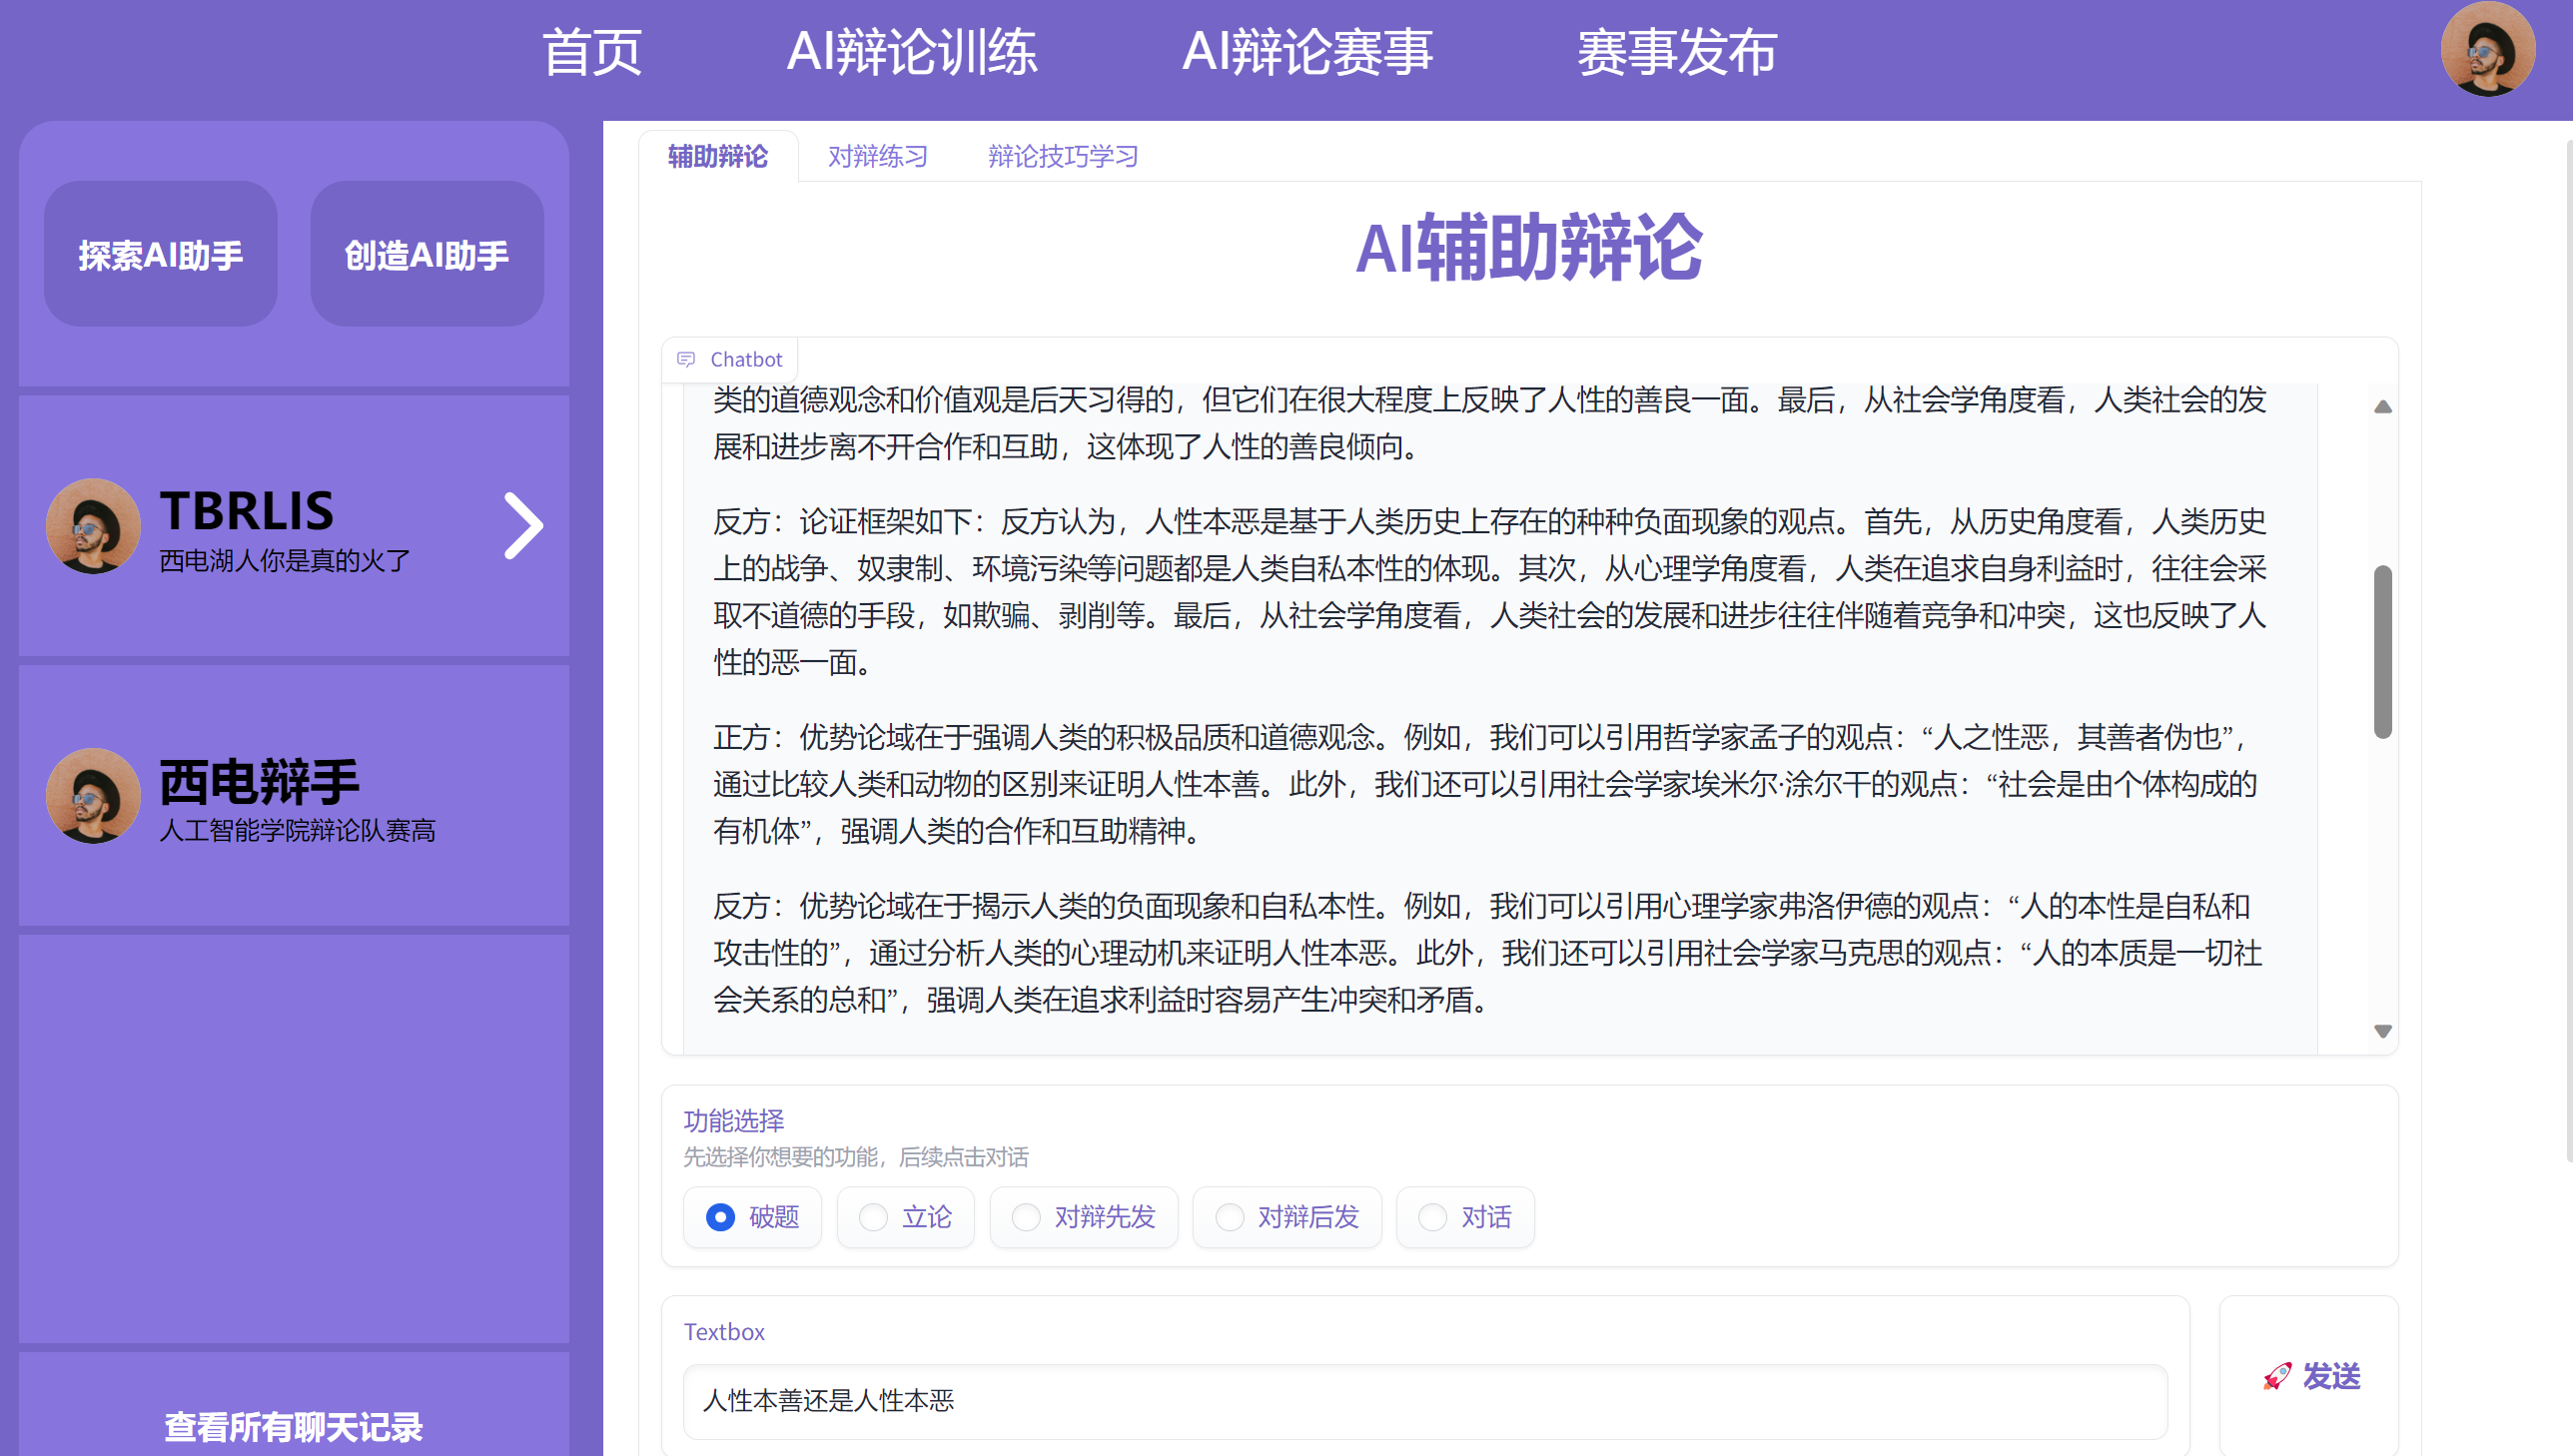
\includegraphics[width=0.8\textwidth,height=0.4\textwidth]{AI辅助破题.png}
      	\caption{AI辩论训练}
      \end{figure} 
        \begin{figure}[H]
      	\centering
      	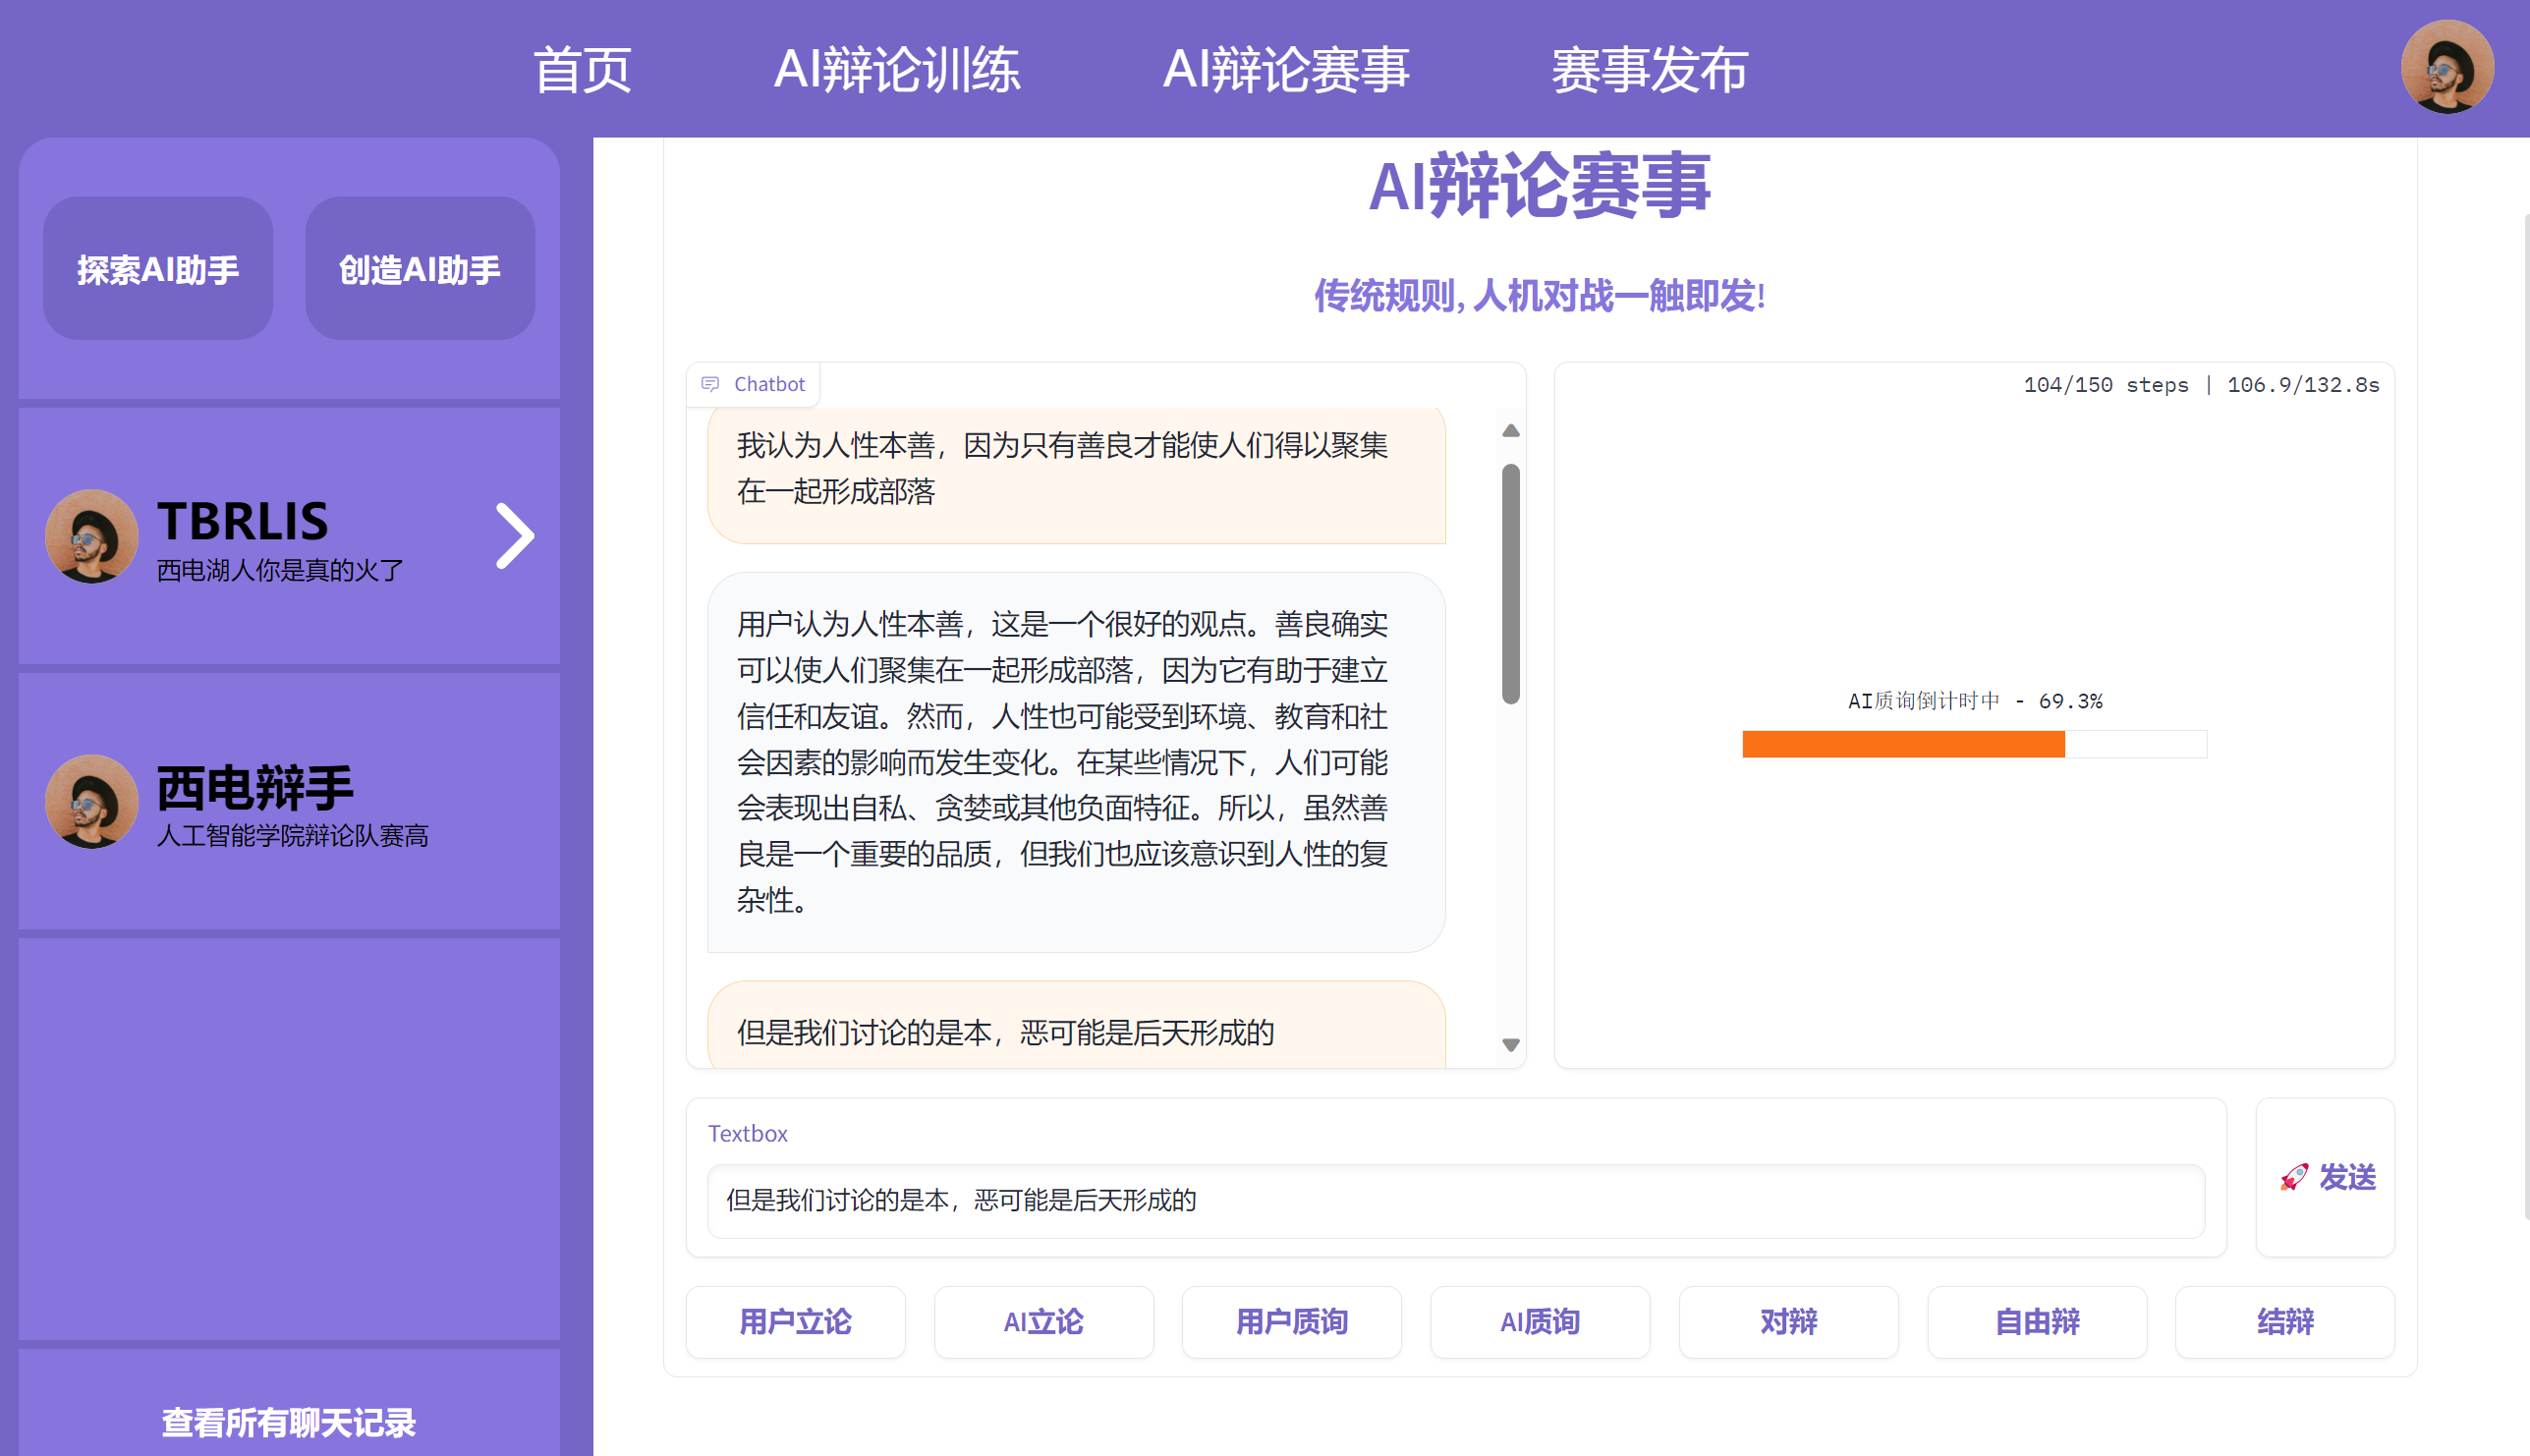
\includegraphics[width=0.8\textwidth,height=0.4\textwidth]{AI赛事质询.png}
      	\caption{AI辩论赛事}
      \end{figure} 
        \begin{figure}[H]
      	\centering
      	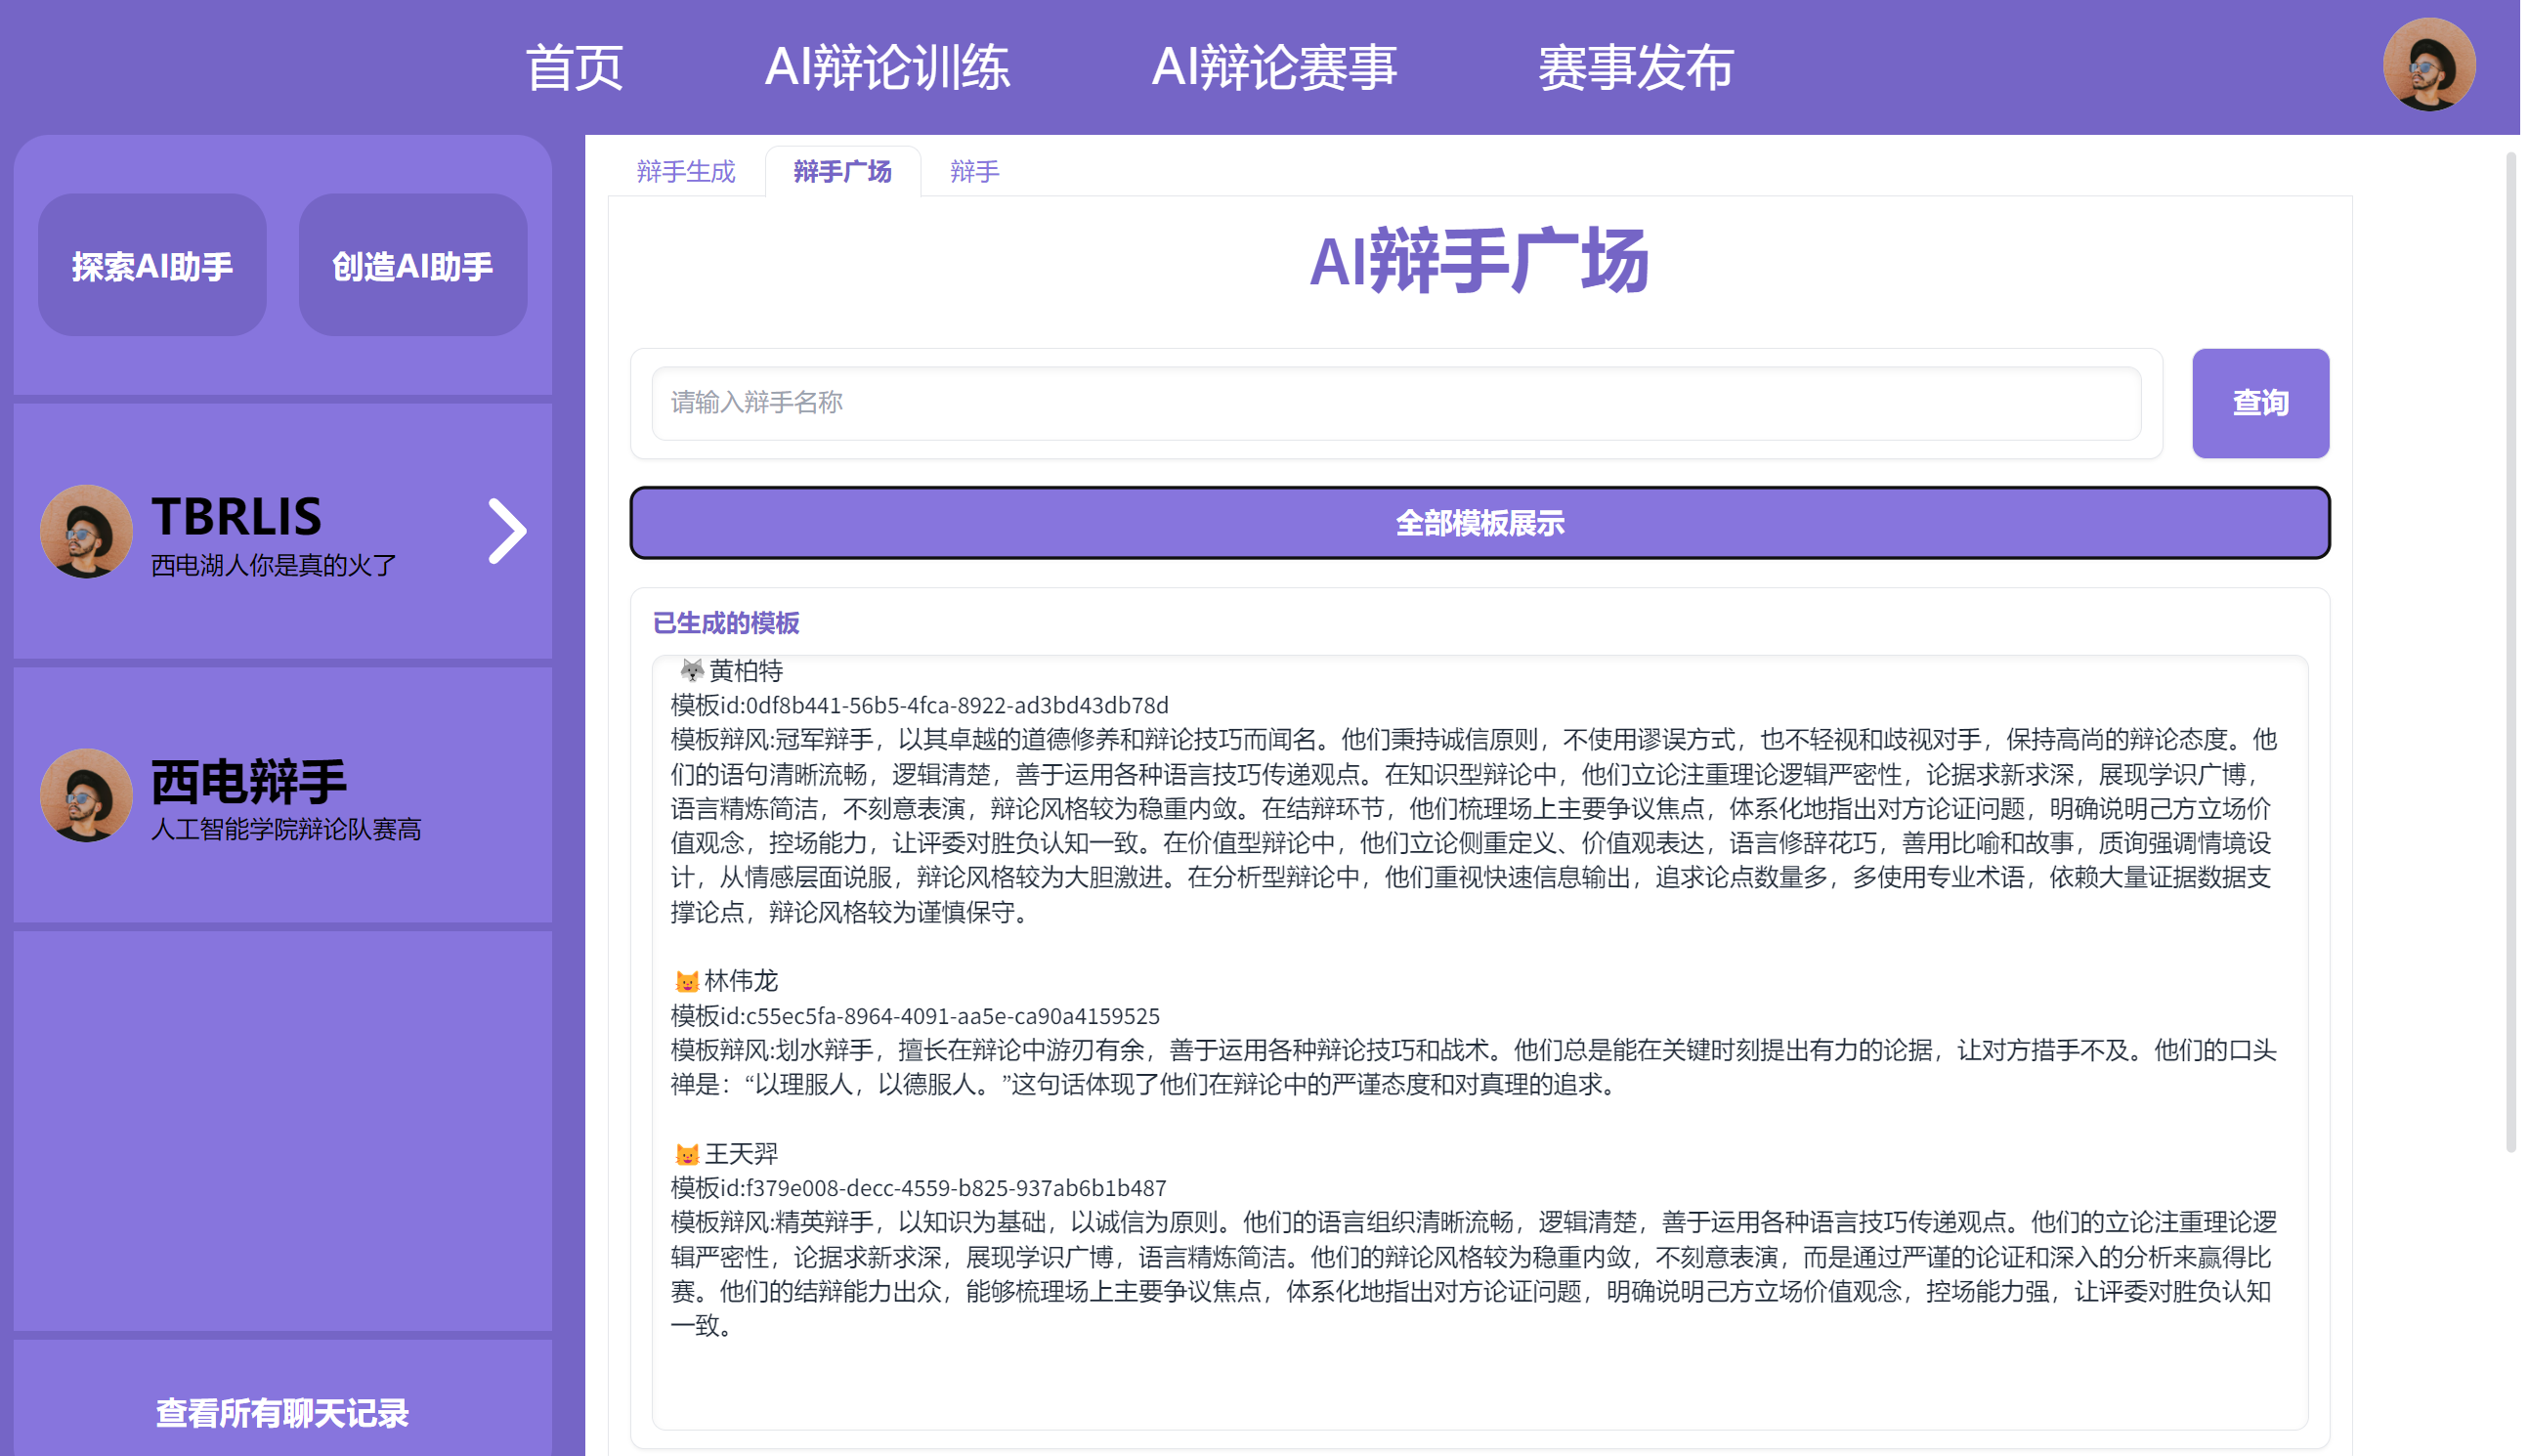
\includegraphics[width=0.8\textwidth,height=0.4\textwidth]{AI辩手广场.png}
      	\caption{AI辩论广场}
      \end{figure} 
        \begin{figure}[H]
      	\centering
      	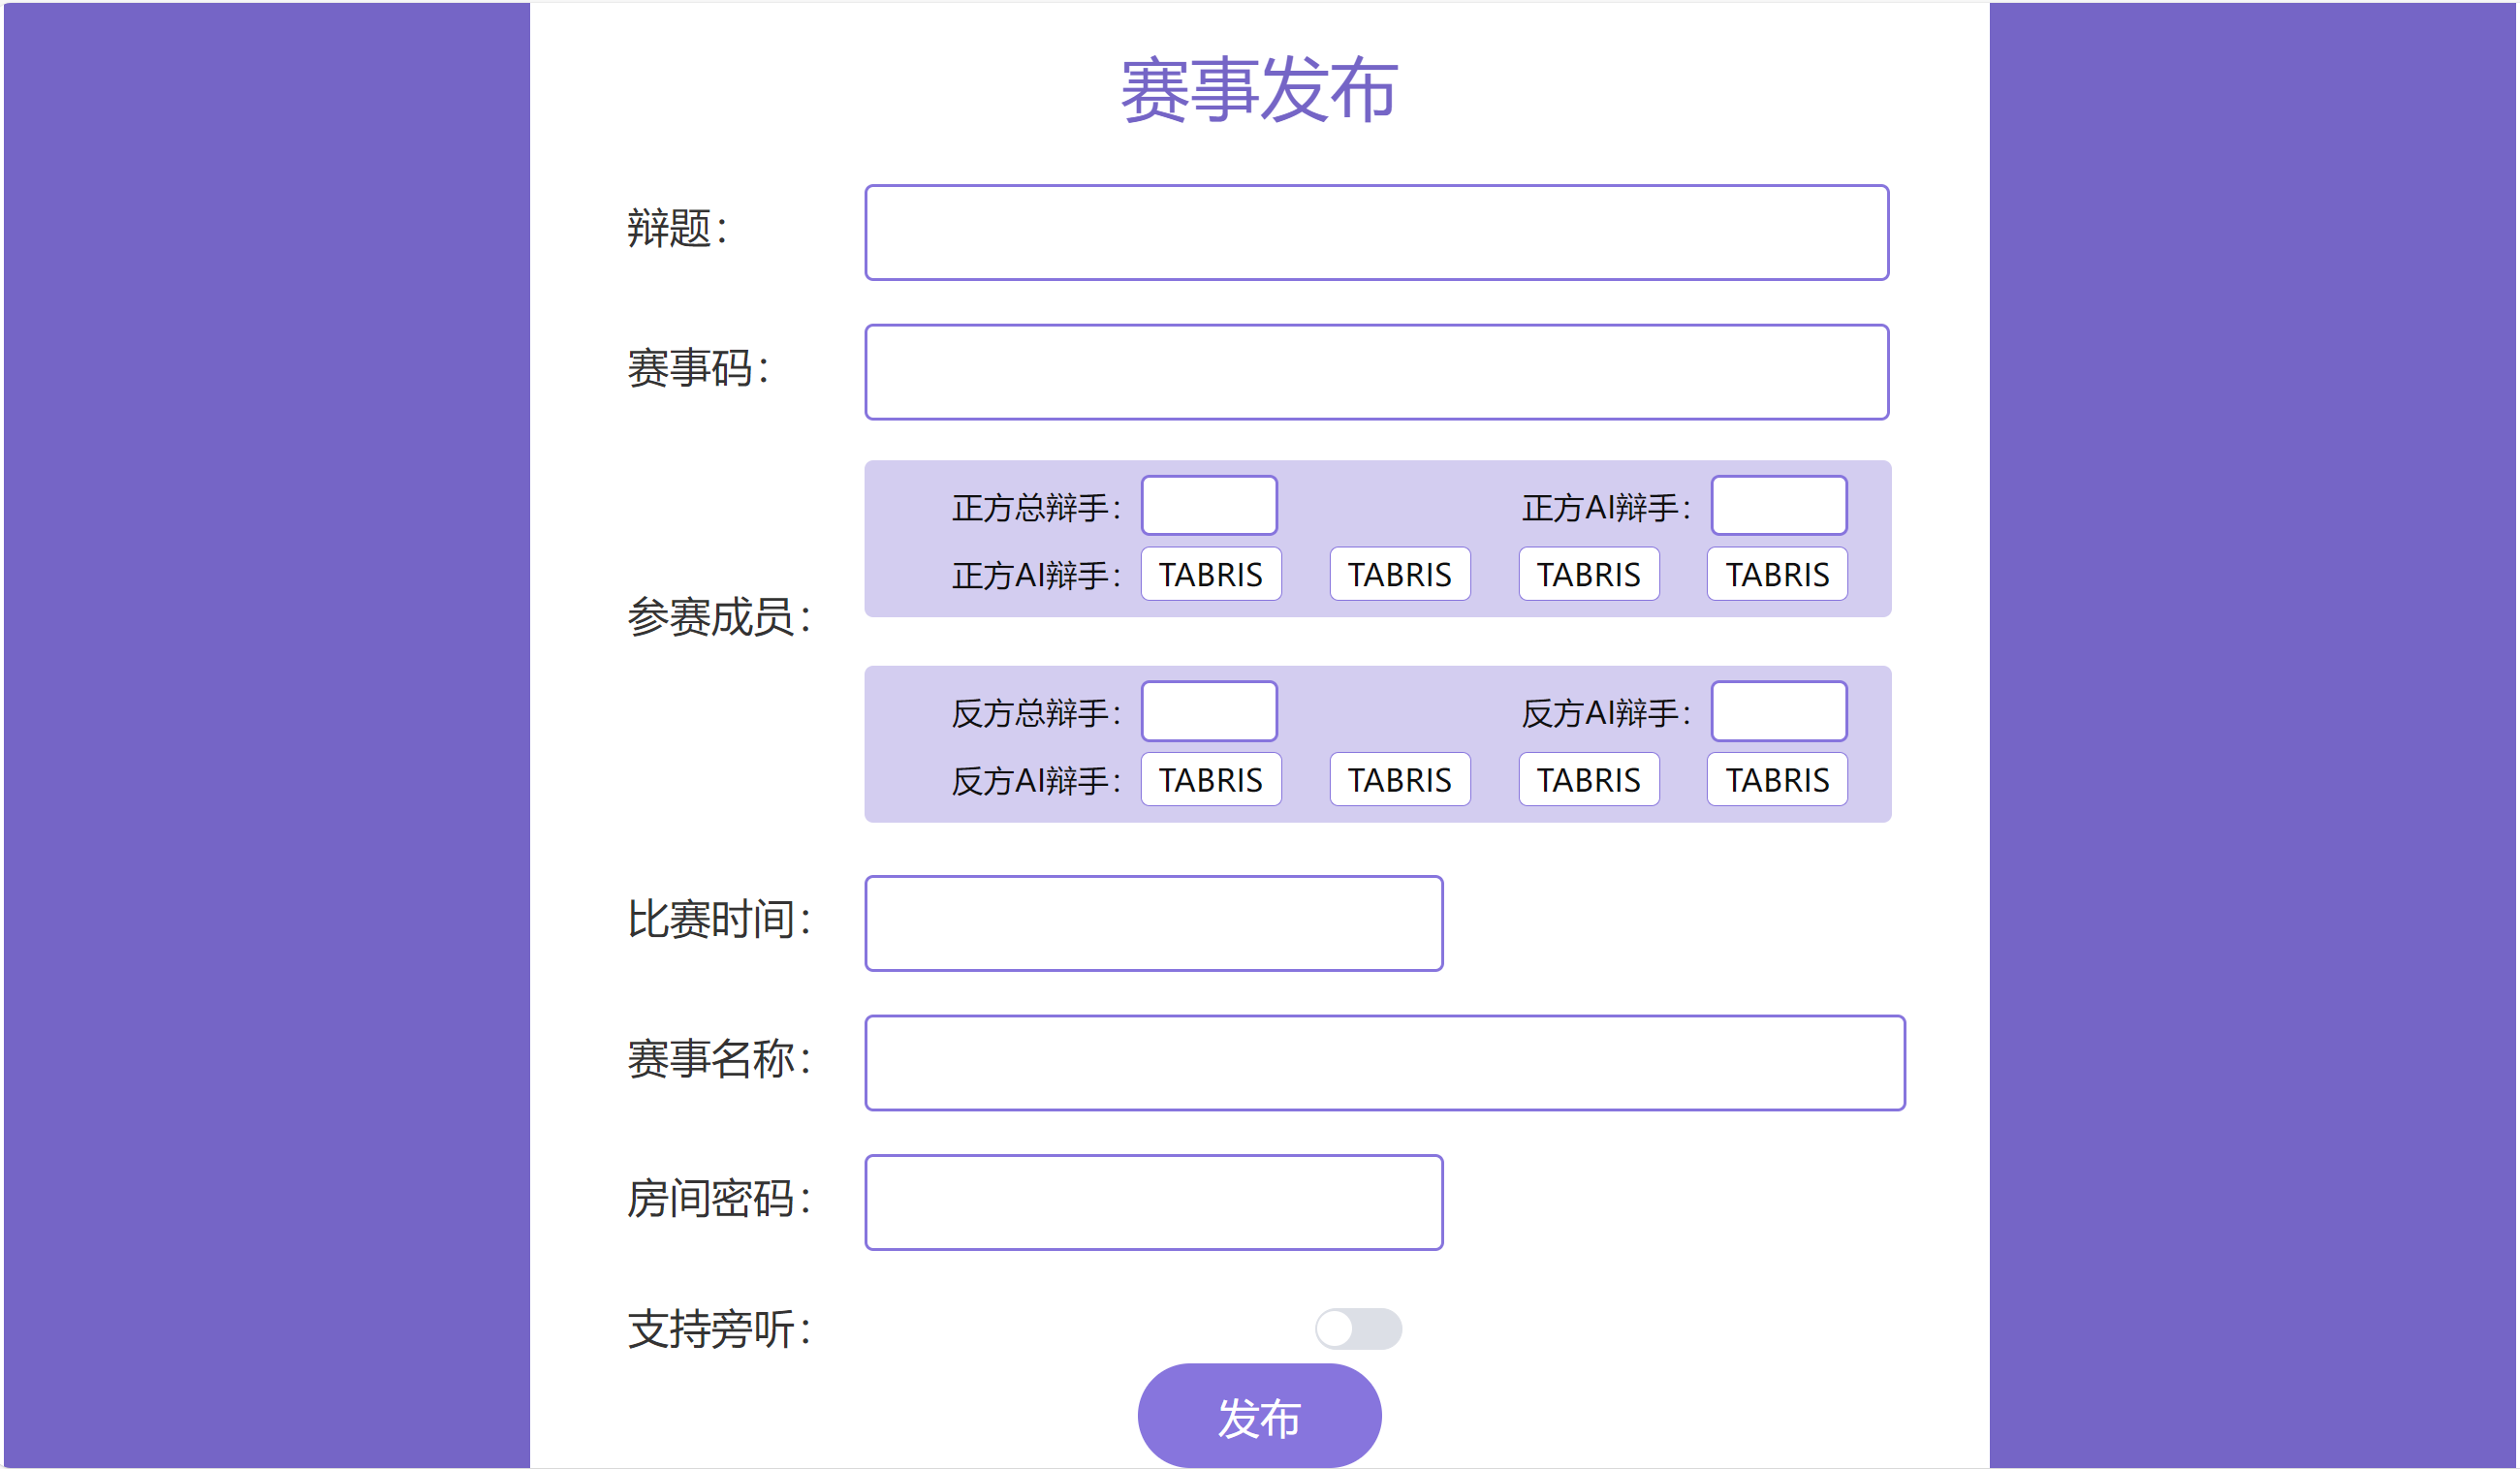
\includegraphics[width=0.8\textwidth,height=0.4\textwidth]{AI赛事发布.png}
      	\caption{赛事发布}
      \end{figure} 
      
        
        \subsection{破题展示}
        \zw{破题功能能从十个不同的辩论角度分析一个辩题,让辩手得以充分了解辩题。}
     	  \begin{figure}[H]
     		\centering
     		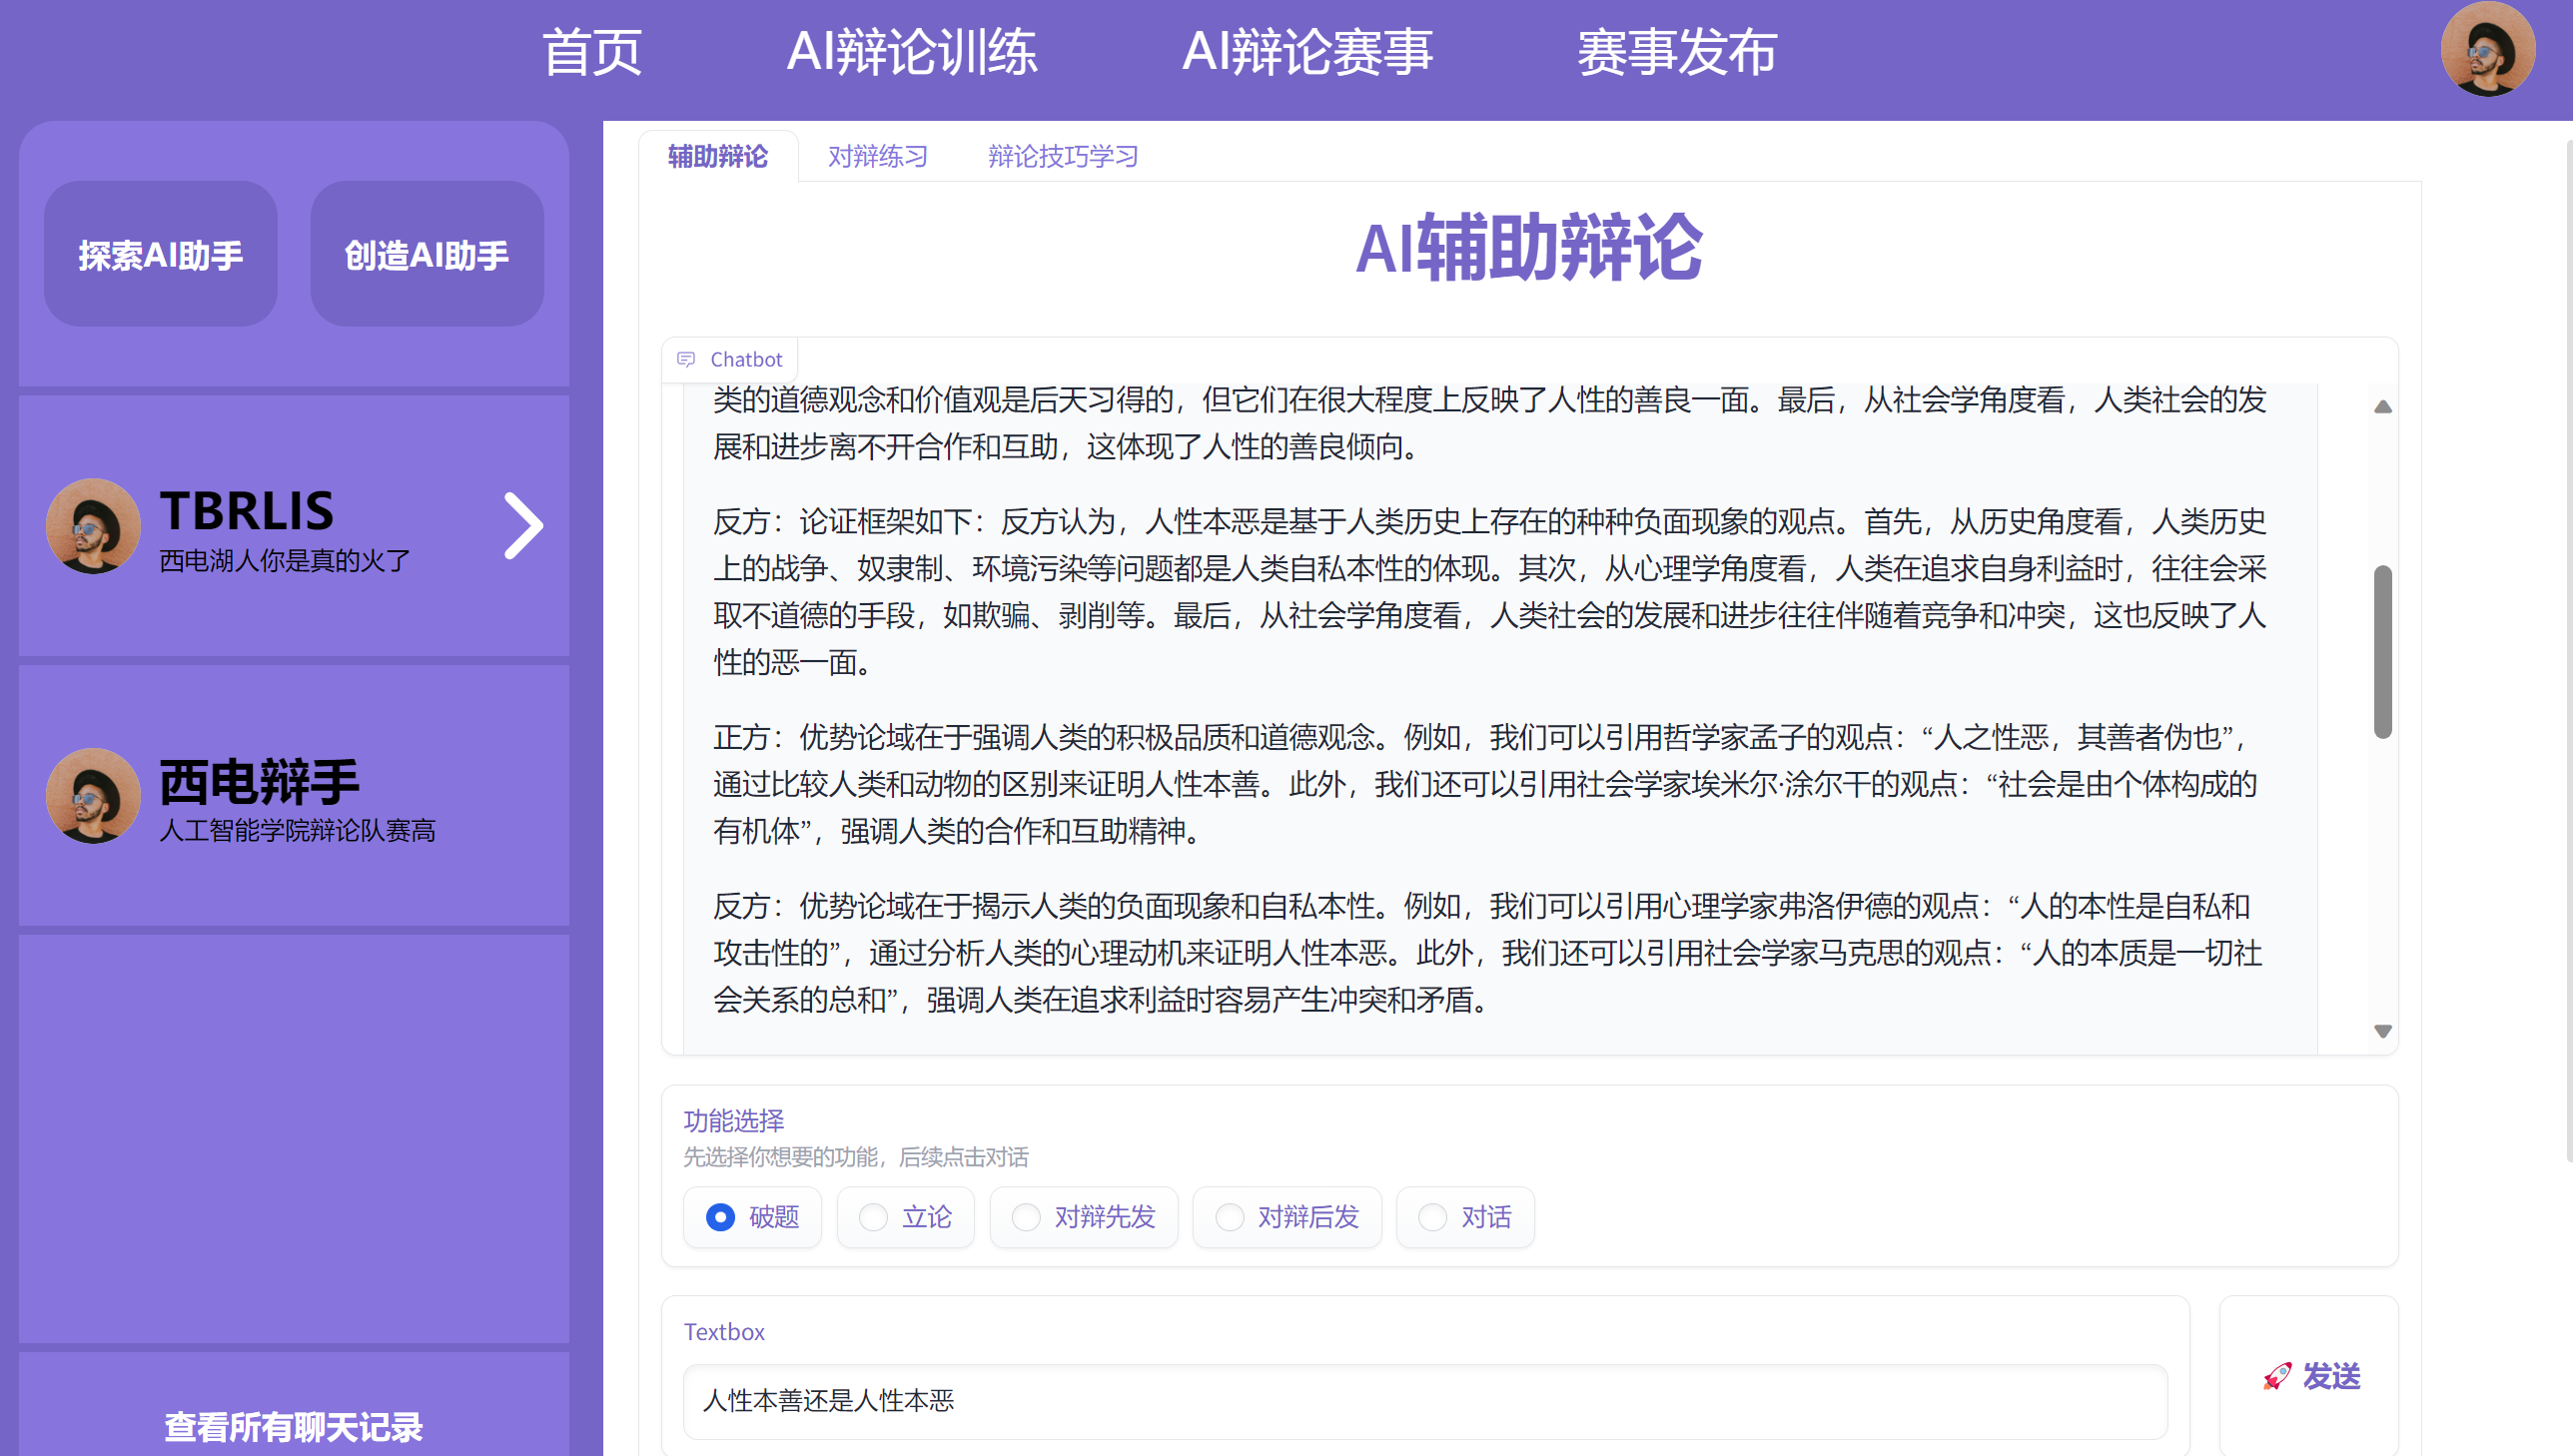
\includegraphics[width=0.8\textwidth,height=0.4\textwidth]{AI辅助破题.png}
     		\caption{AI破题展示}
     	\end{figure} 
        
        \subsection{立论展示}
         \zw{立论功能基本能输出一篇字数达标且格式符合要求,论证质量过关的辩论稿。}
     
         \begin{figure}[H]
        	\centering
        	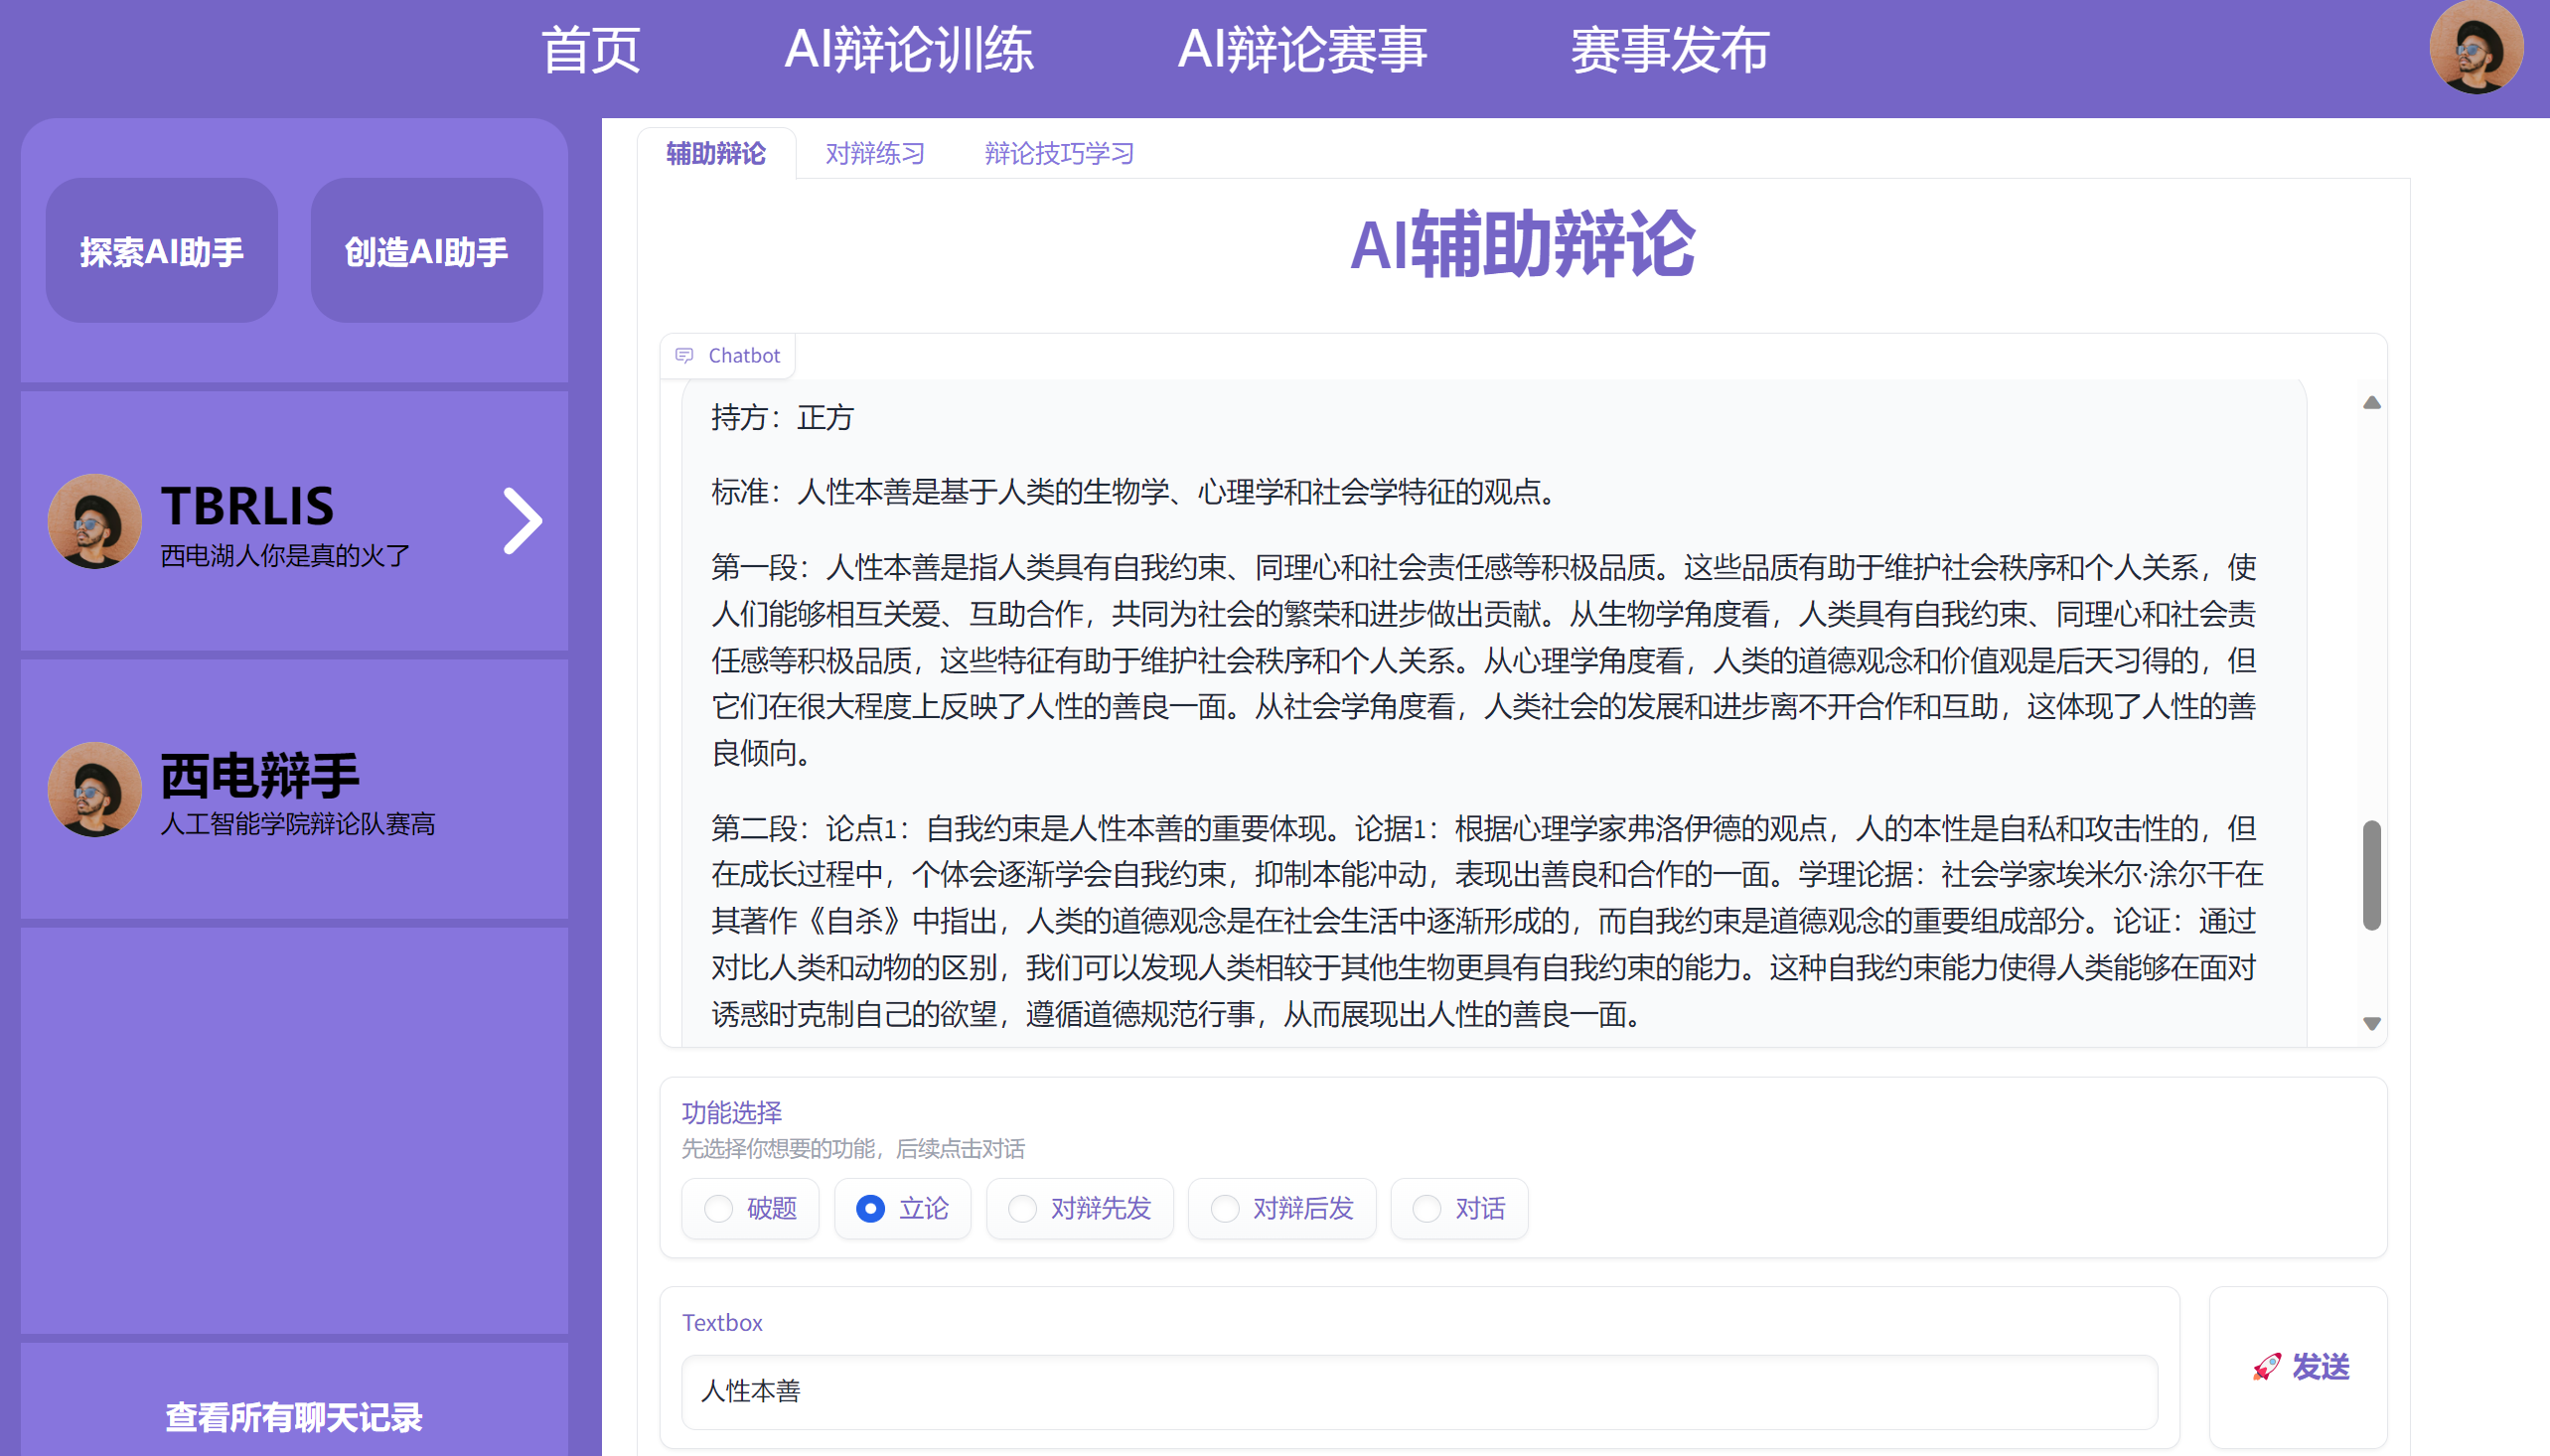
\includegraphics[width=0.8\textwidth,height=0.4\textwidth]{AI辅助立论.png}
        	\caption{AI立论展示}
        \end{figure} 
        \subsection{对话展示}
        \zw{对话功能充分调用了星火大模型V2的能力,通过与大模型进行聊天,了解辩题相关的信息和学理。}
        
        \begin{figure}[H]
        	\centering
        	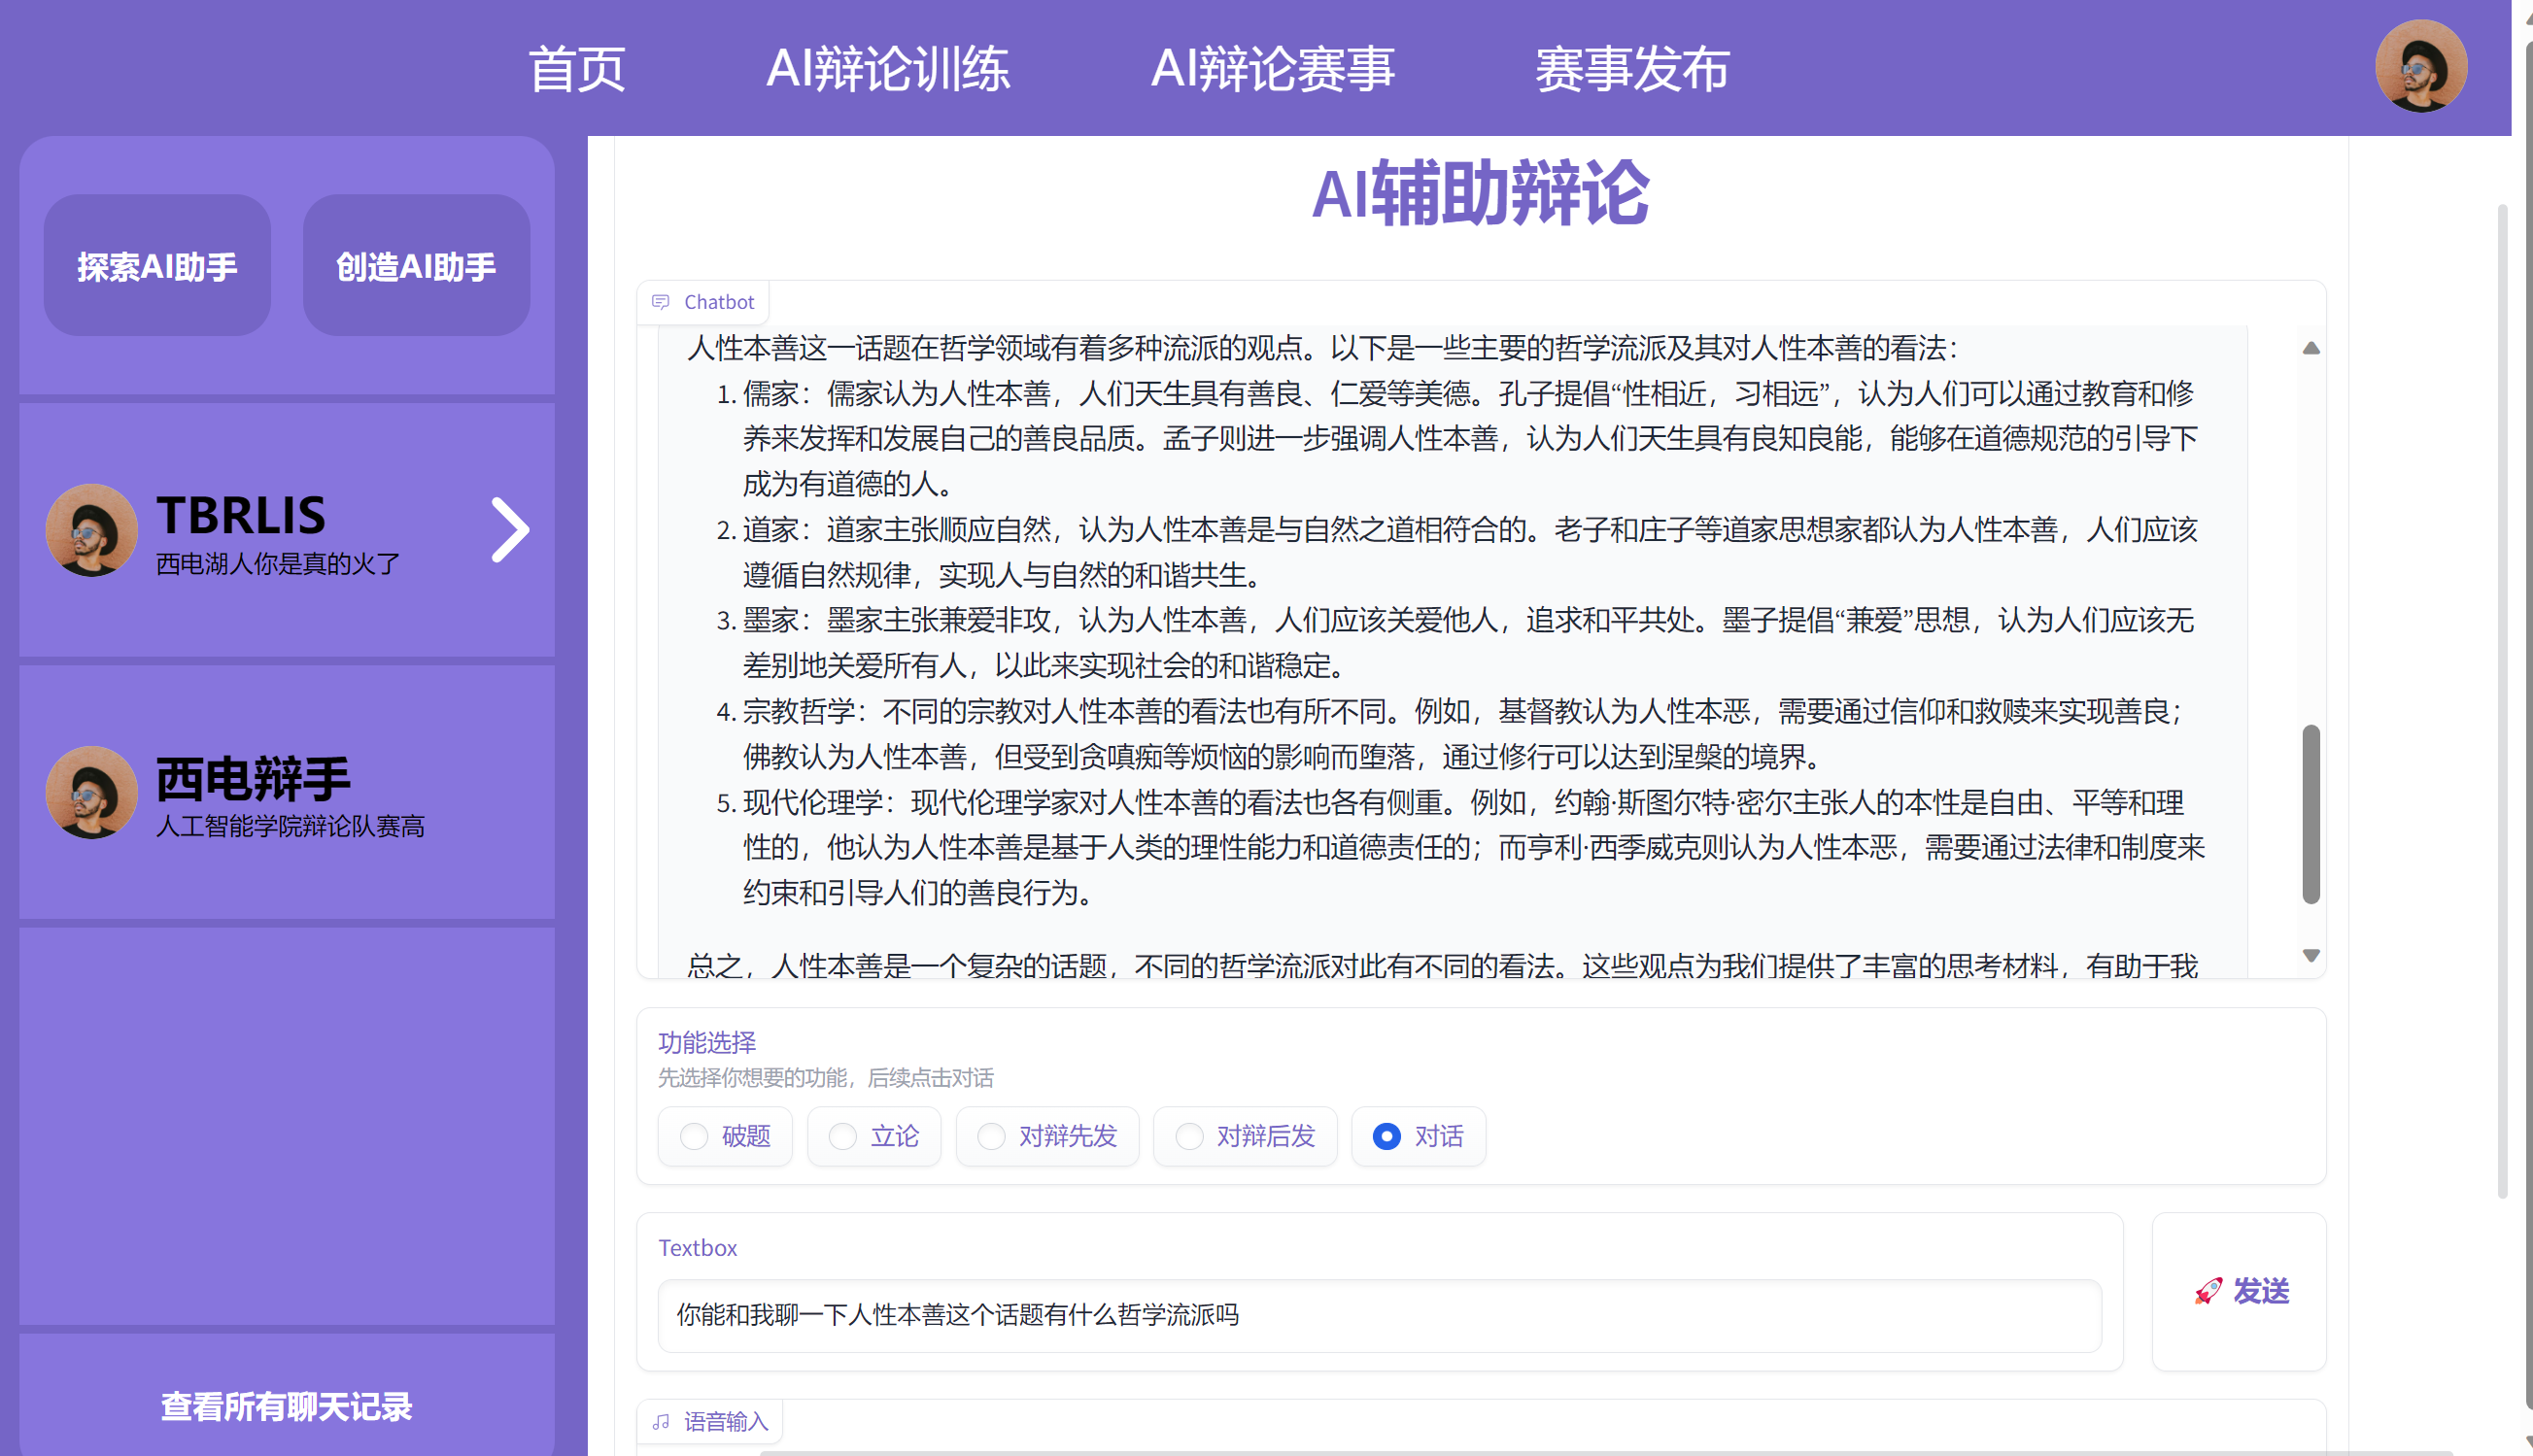
\includegraphics[width=0.8\textwidth,height=0.4\textwidth]{AI辅助对话.png}
        	\caption{AI对话展示}
        \end{figure} 
        
        
        \subsection{AI对辩}
        \zw {对辩分为练习和总结三个部分,在练习部分,我们输入了一段文稿,SparkDebate会对我们的陈述进行了针锋相对的反驳,我们可以针对反驳与它进行多轮对话。在总结部分,SparkDebate会对对辩全部过程进行总结,并对我们的辩论水平做出了评价给出了等级,最后还会给出了相应的提升建议。}
      
        
        \subsubsection{对辩练习}
         \begin{figure}[H]
        	\centering
        	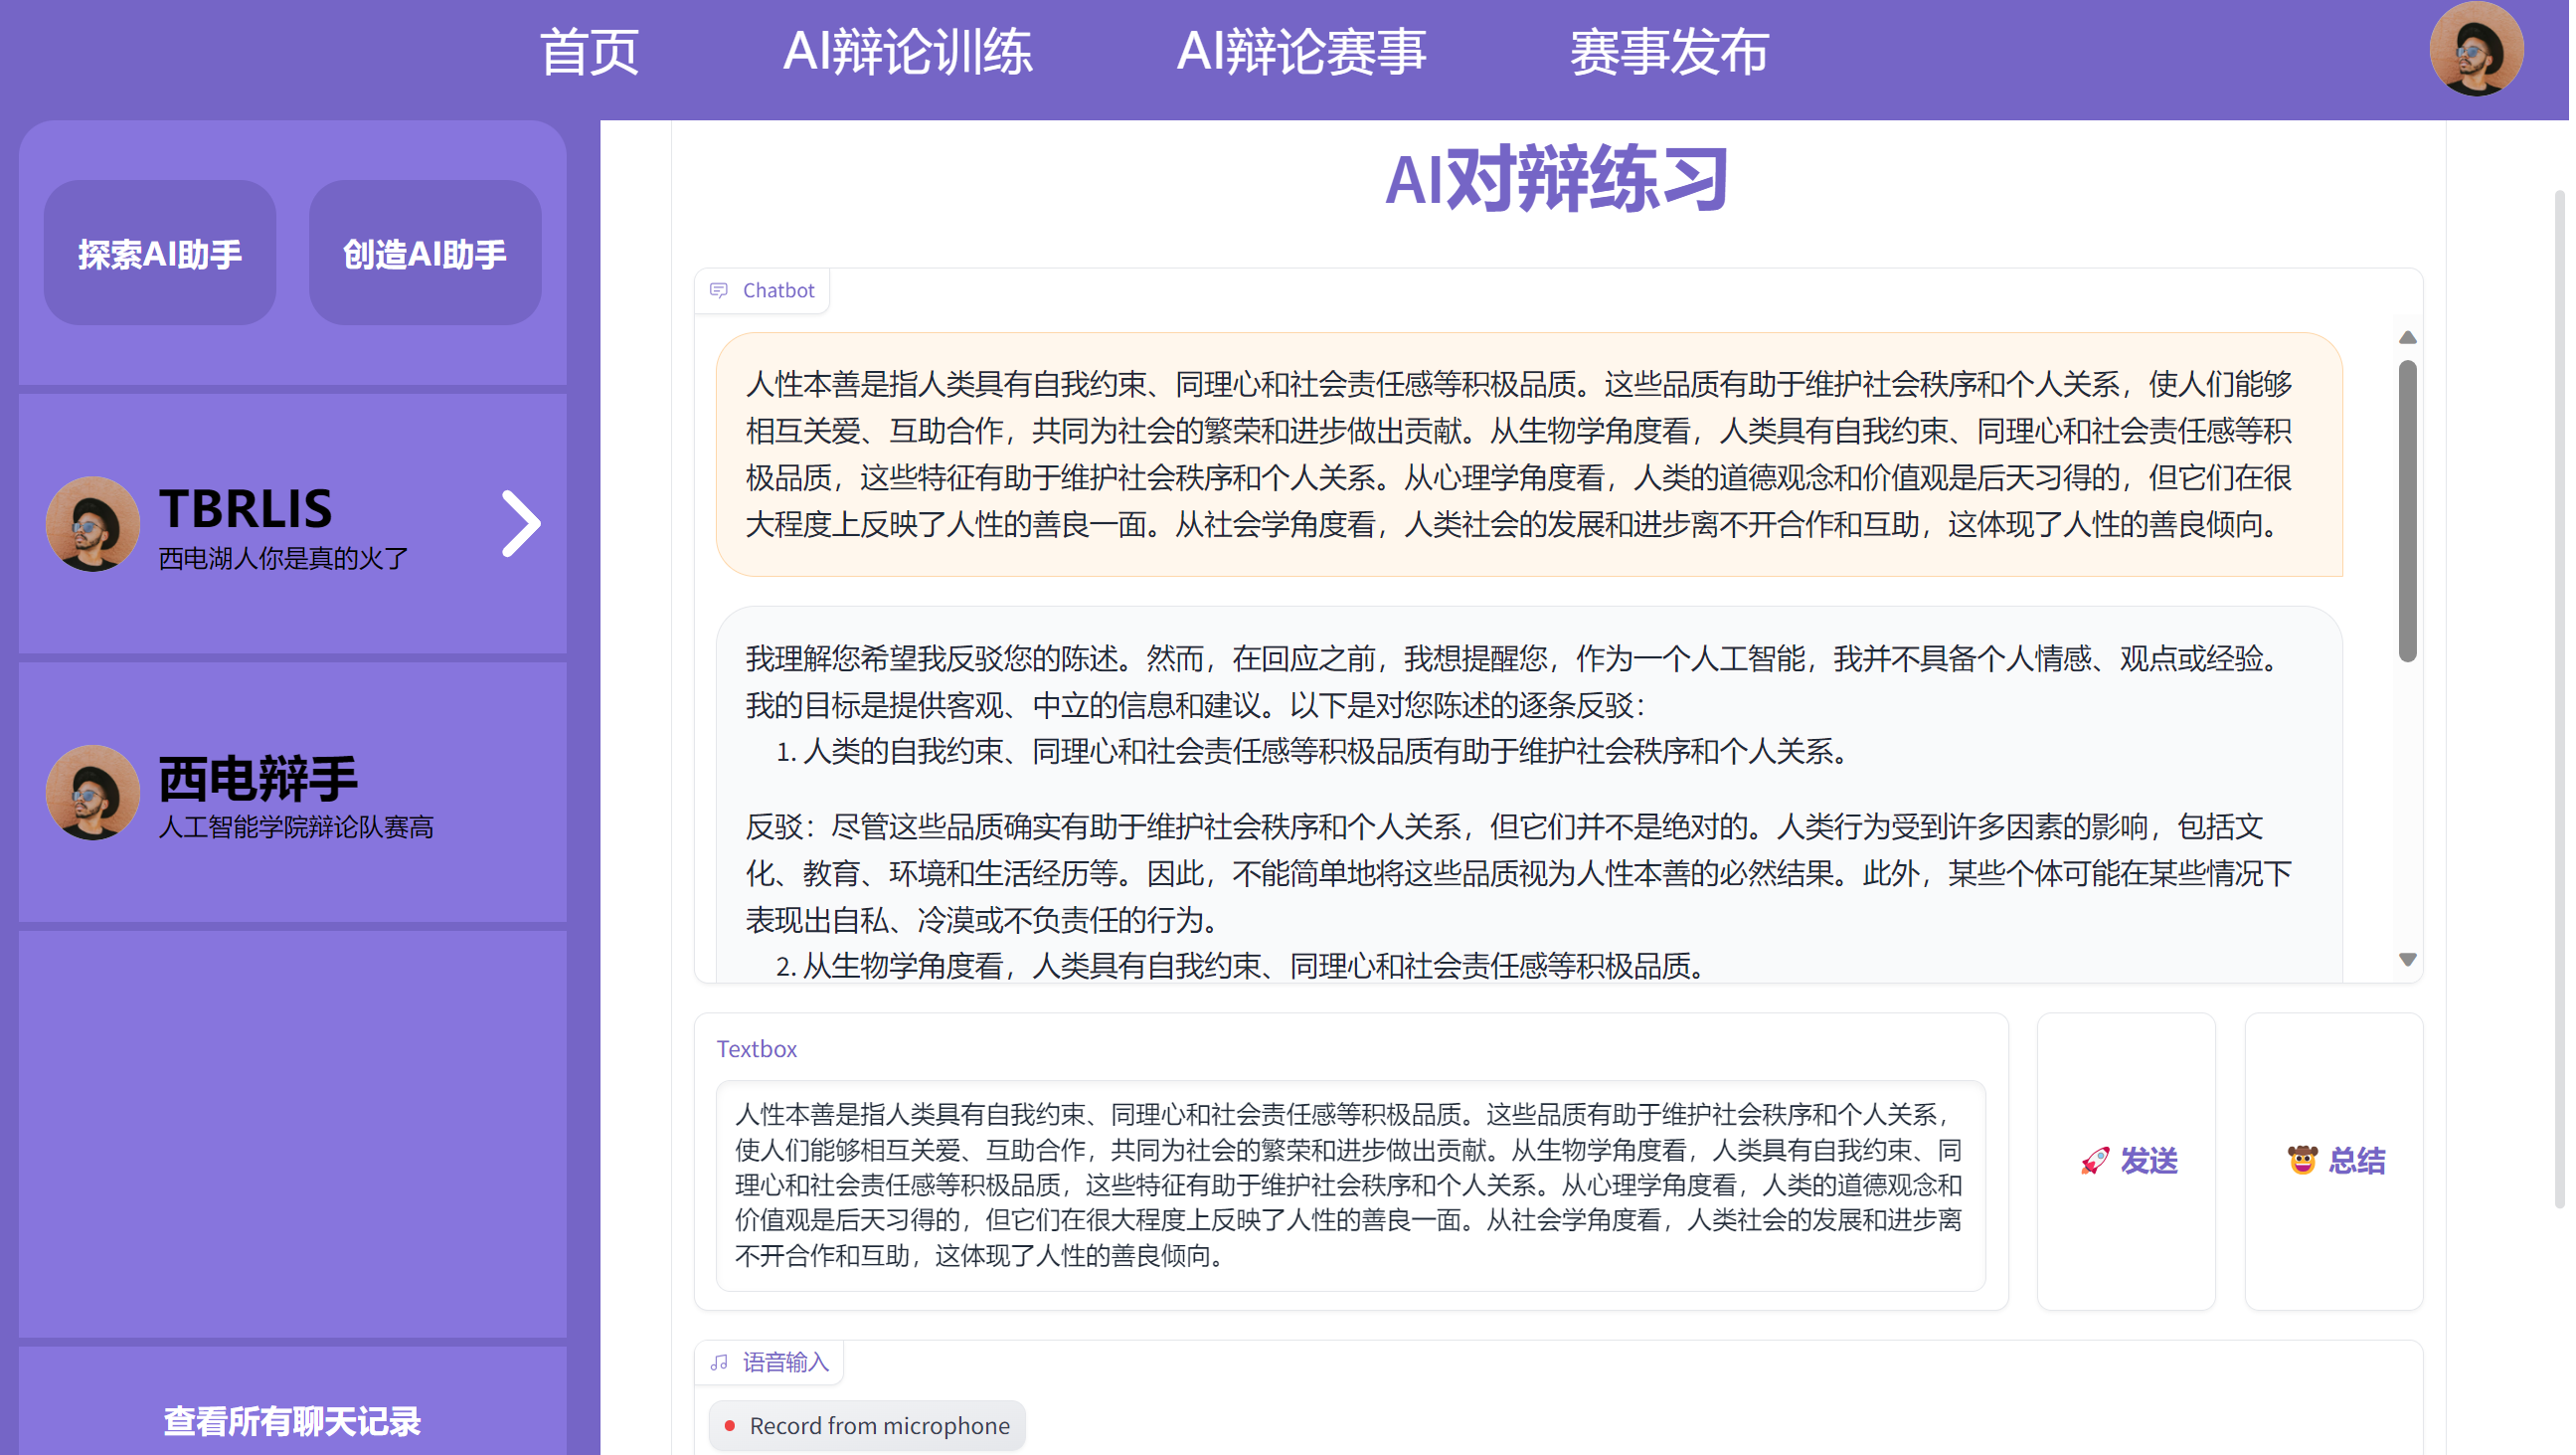
\includegraphics[width=0.8\textwidth,height=0.4\textwidth]{AI对辩练习.png}
        	\caption{ 对辩效果展示}
        \end{figure} 
        
    
        
        \subsubsection{对辩总结}
         \begin{figure}[H]
        	\centering
        	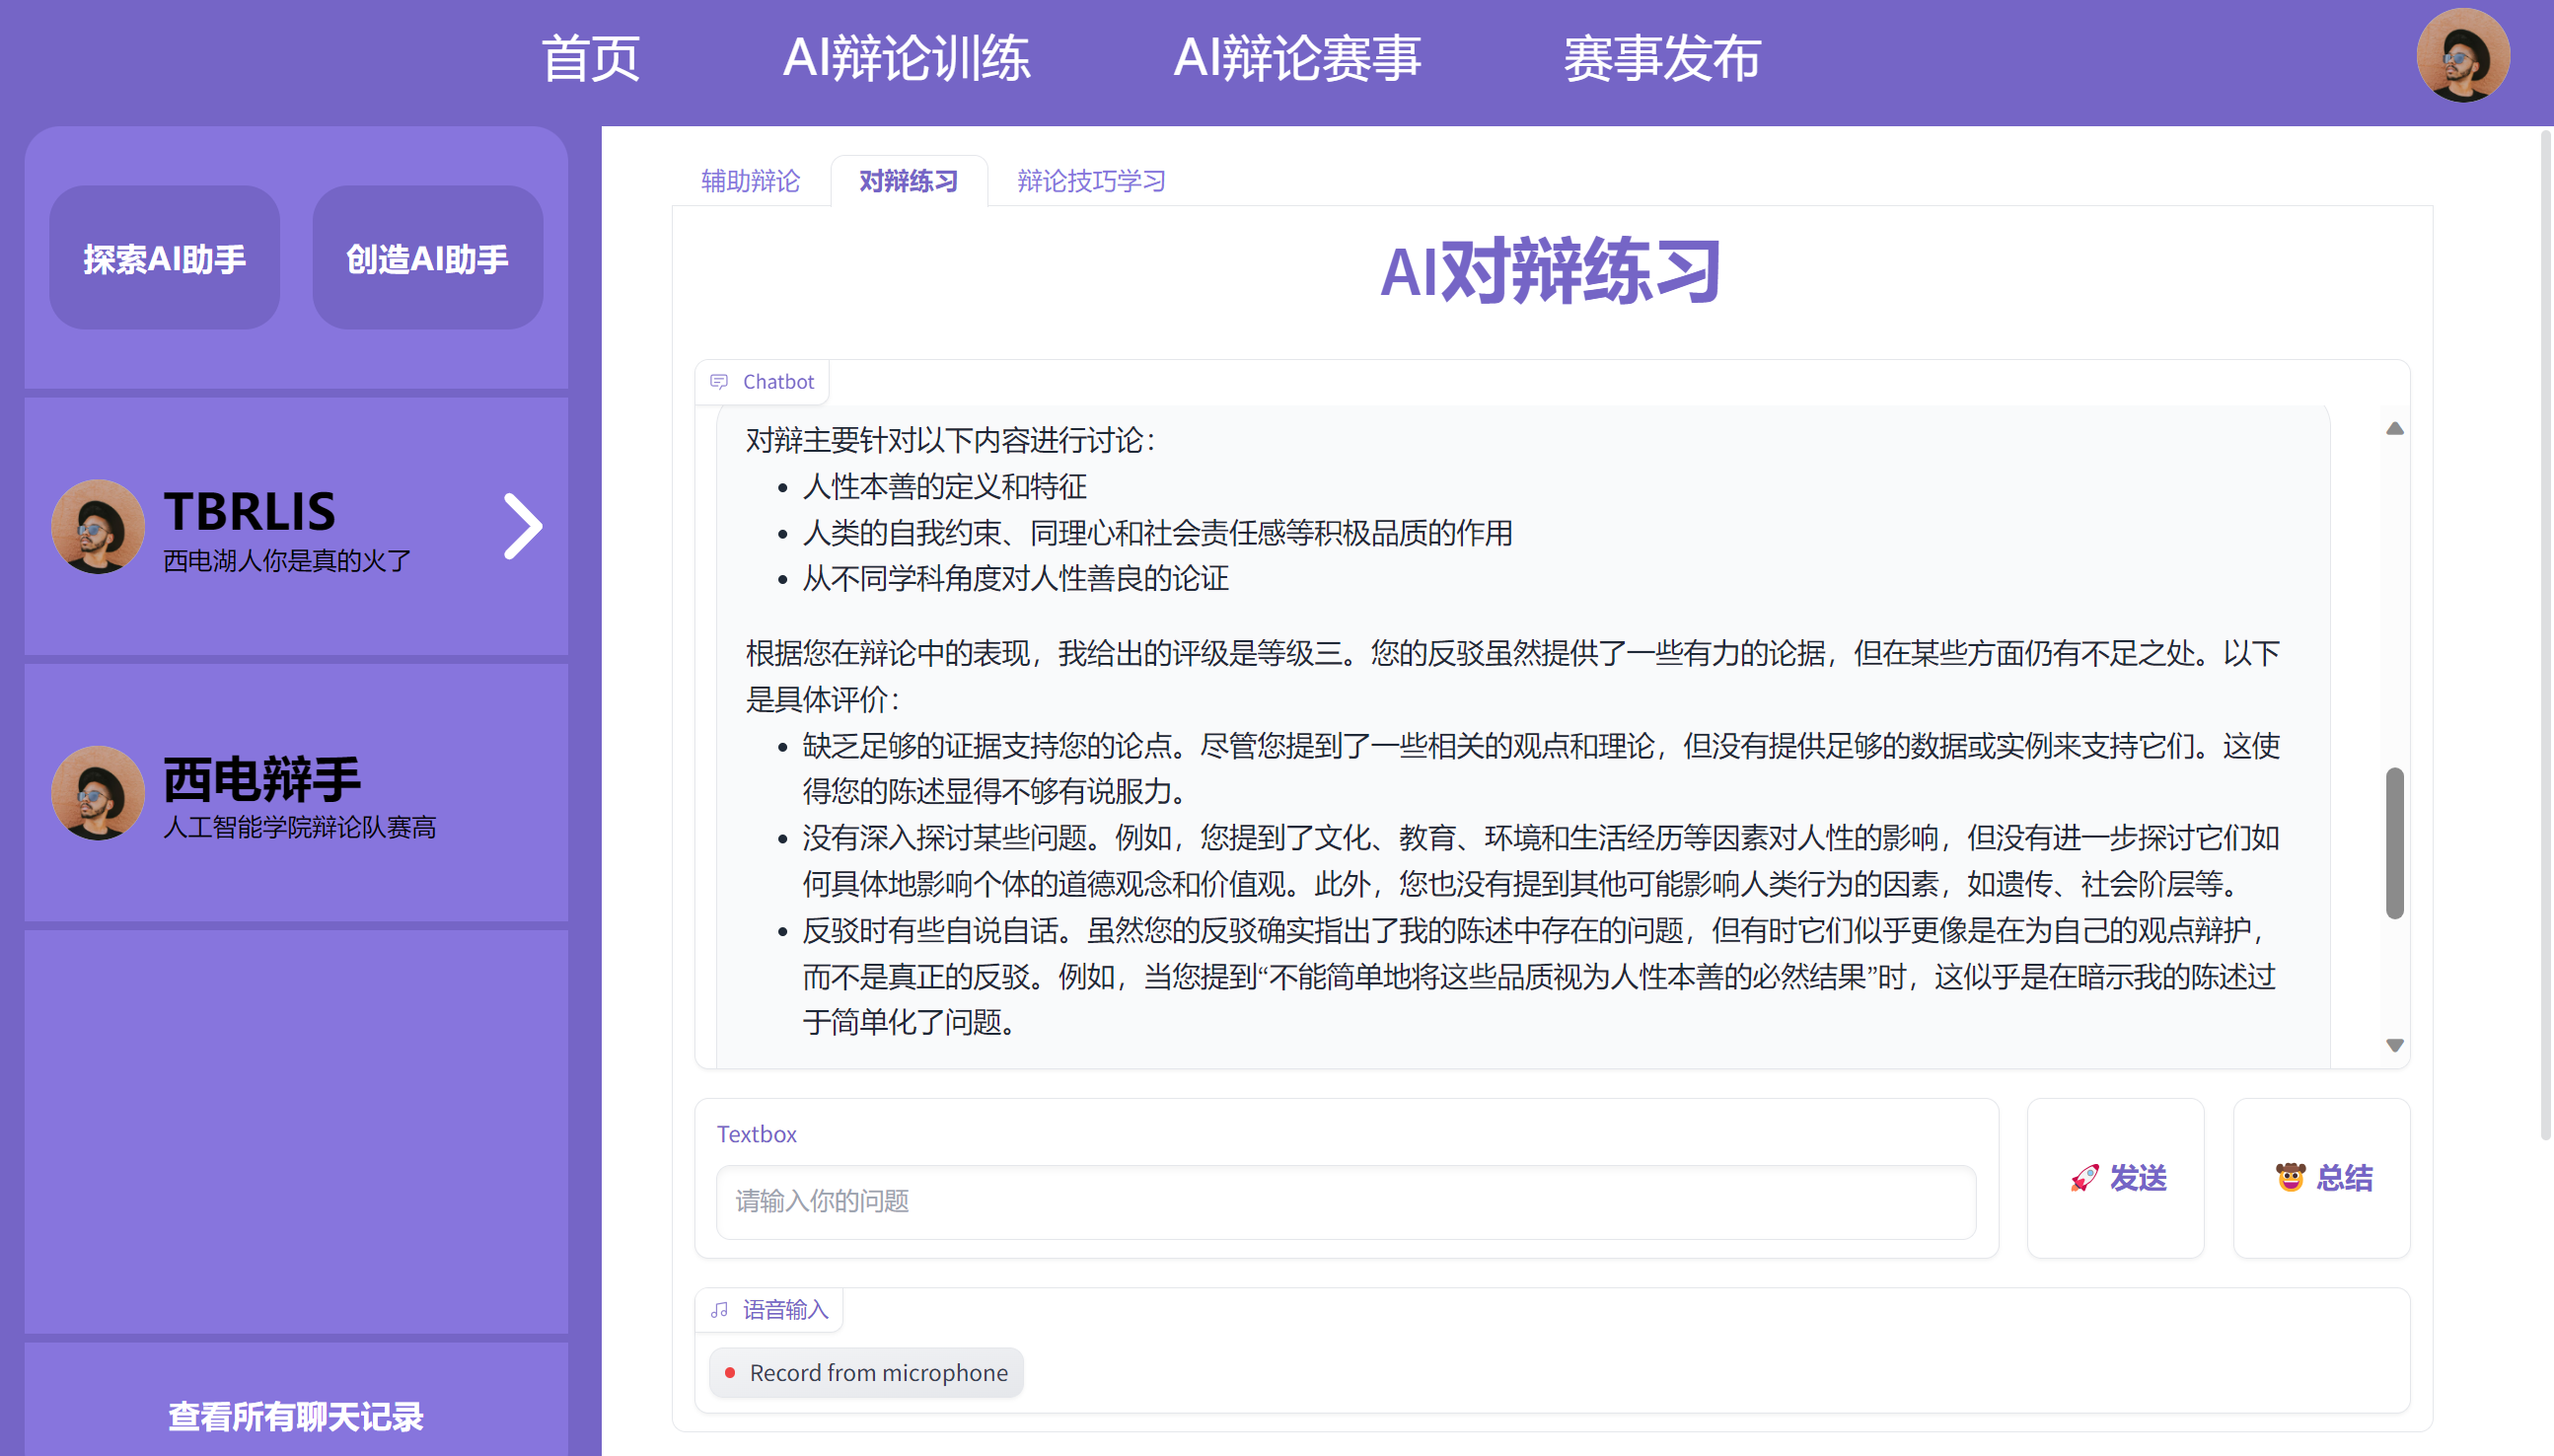
\includegraphics[width=0.8\textwidth,height=0.4\textwidth]{AI对辩总结.png}
        	\caption{对辩总结效果展示}
        \end{figure} 
        
        \subsection{AI经典辩论赛事}
        \zw{在AI辩论赛事部分,我们展现了全流程的辩论能力。}
          \begin{figure}[H]
        	\centering
        	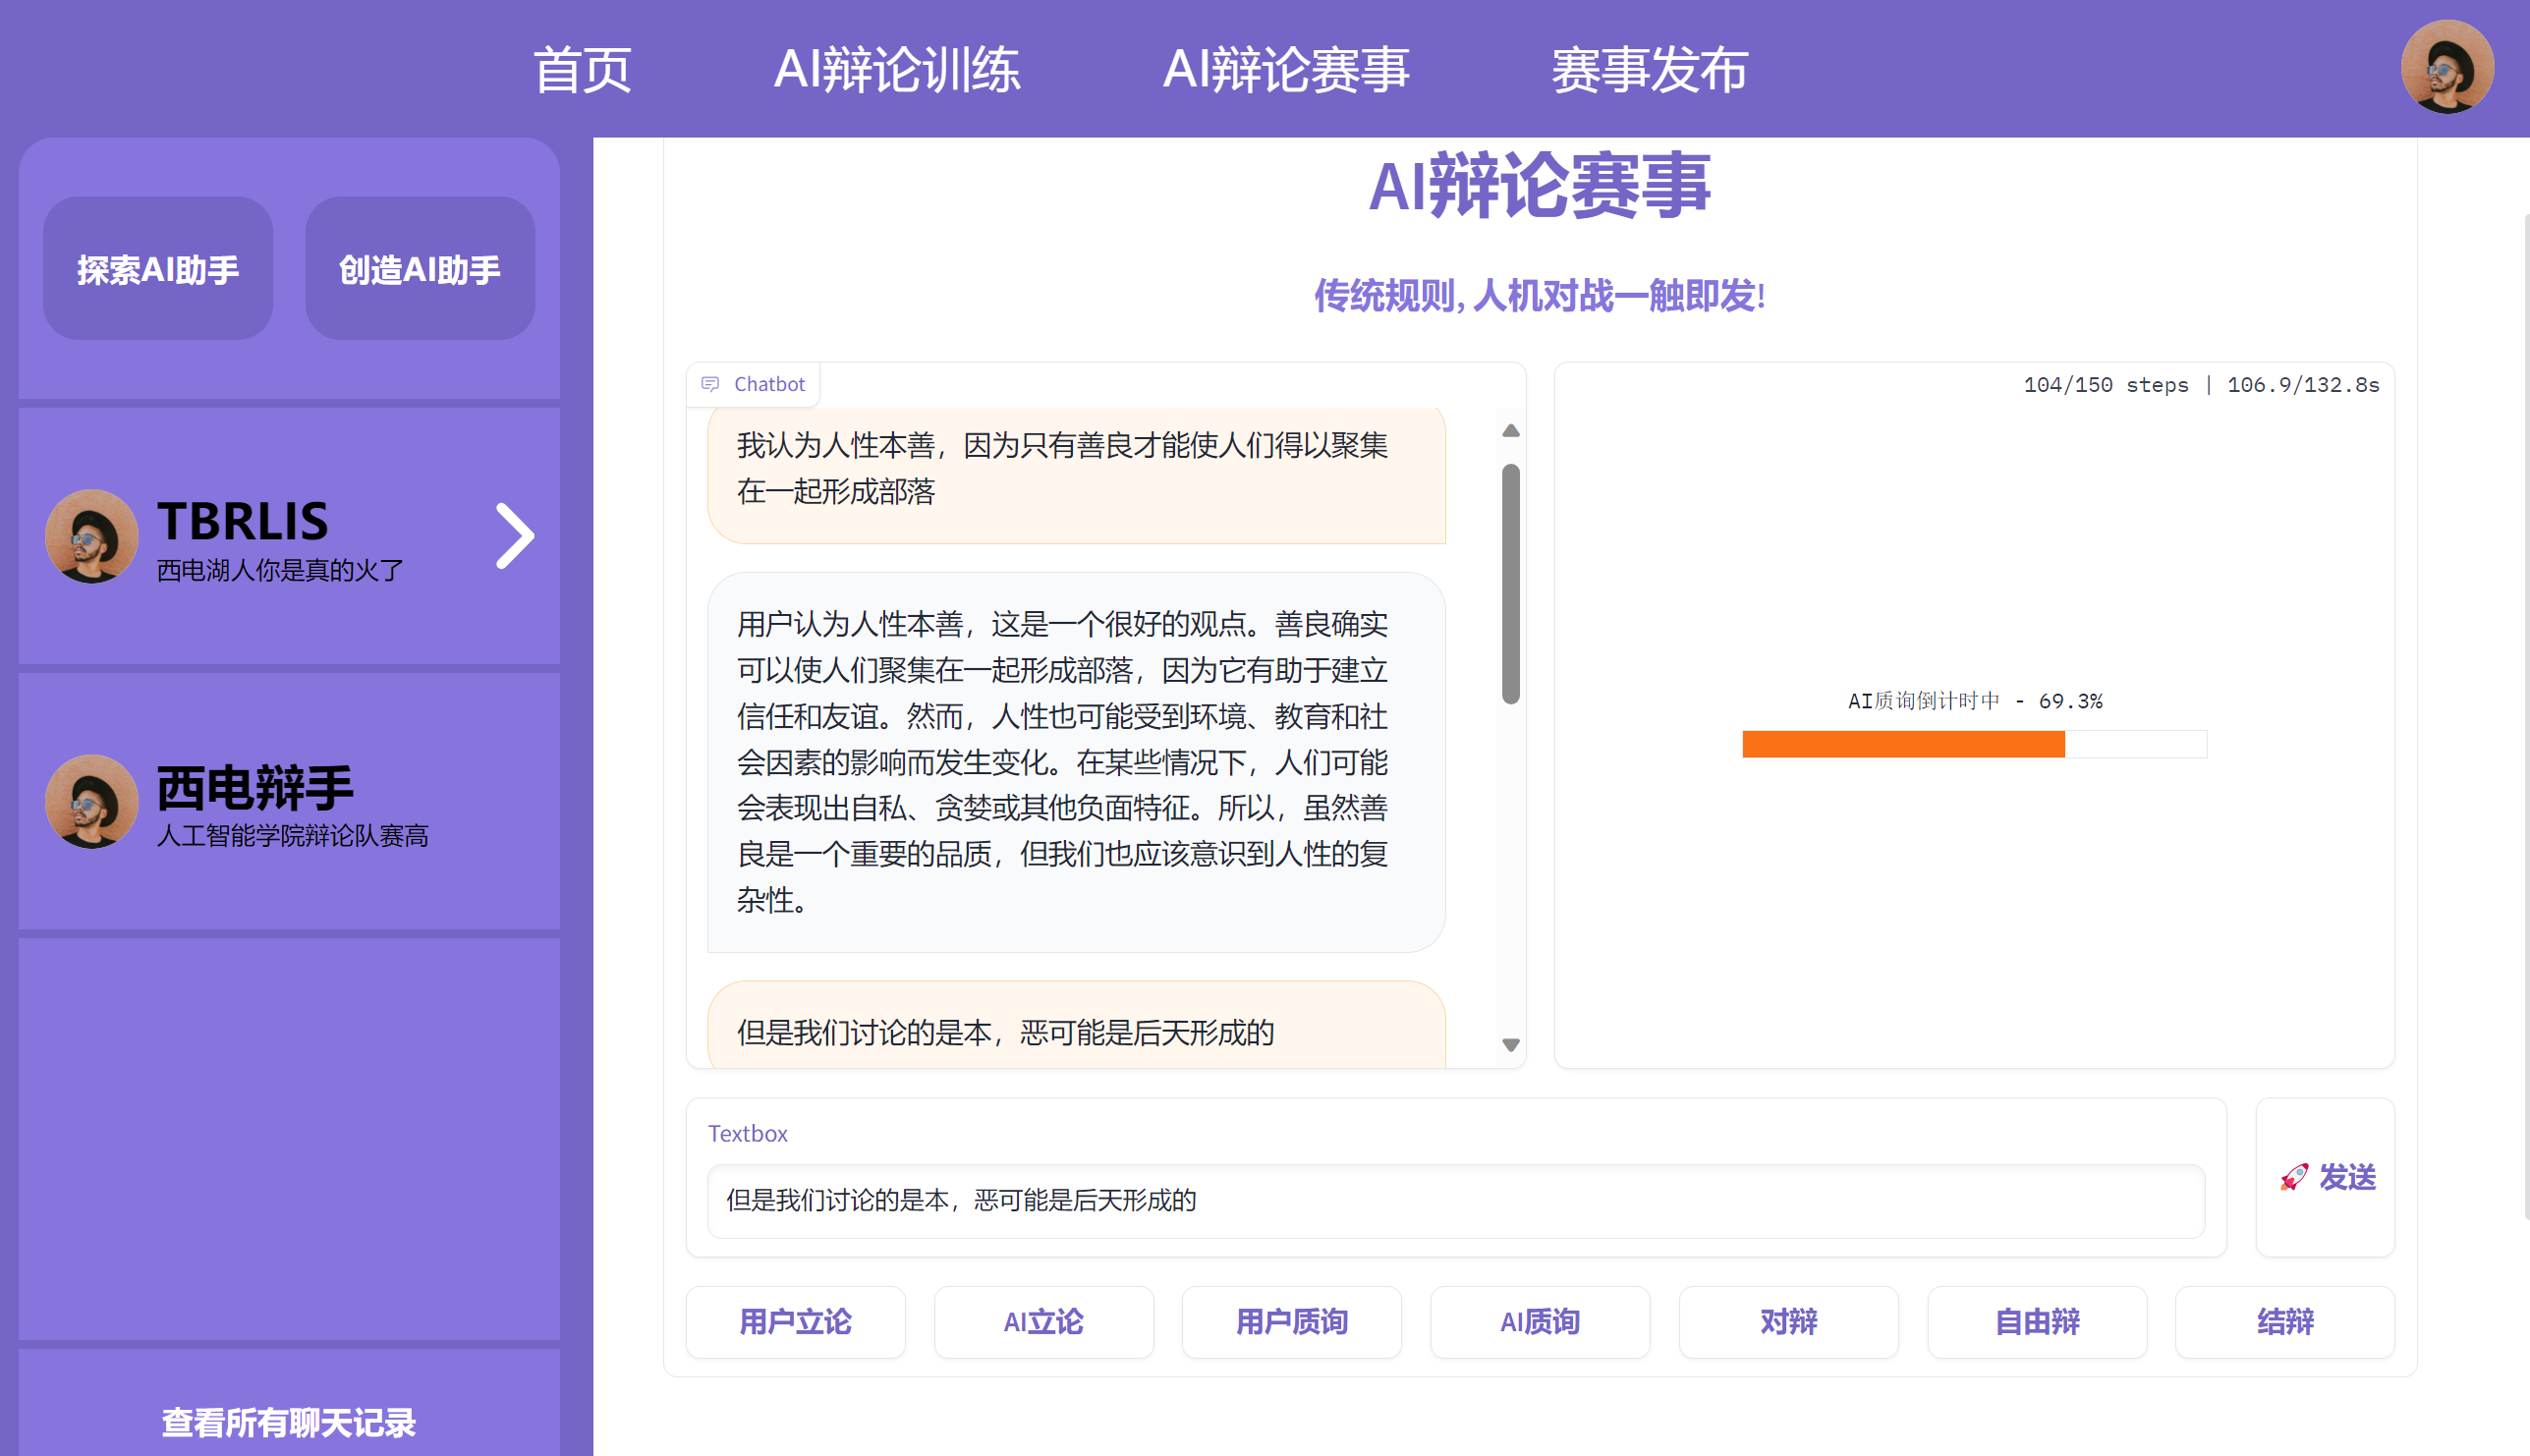
\includegraphics[width=0.8\textwidth,height=0.4\textwidth]{AI赛事质询.png}
        	\caption{赛事质询}
        \end{figure} 
        
        \subsection{AI关卡自定义}
        \zw{在AI关卡自定义部分,我们上传了一份辩论文字资料,随后AI辩手的回答与论点就会高度运用上文字资料的内容。}
          \begin{figure}[H]
        	\centering
        	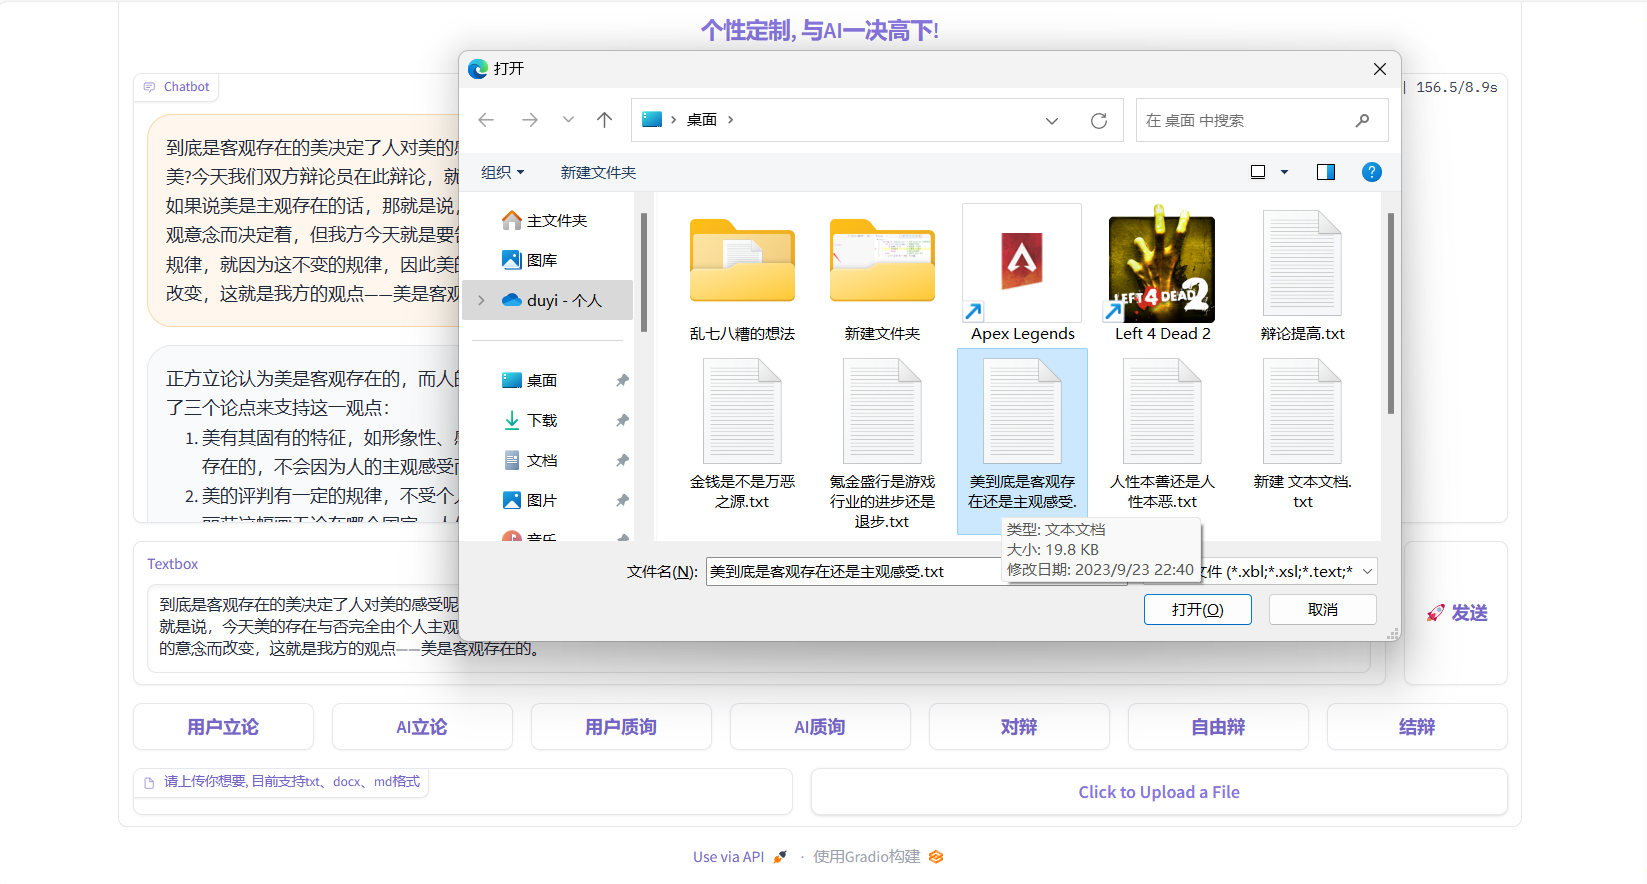
\includegraphics[width=0.8\textwidth,height=0.4\textwidth]{AI自定义上传.png}
        	\caption{文字资料上传}
        \end{figure} 
   
        \begin{figure}[H]
        	\centering
        	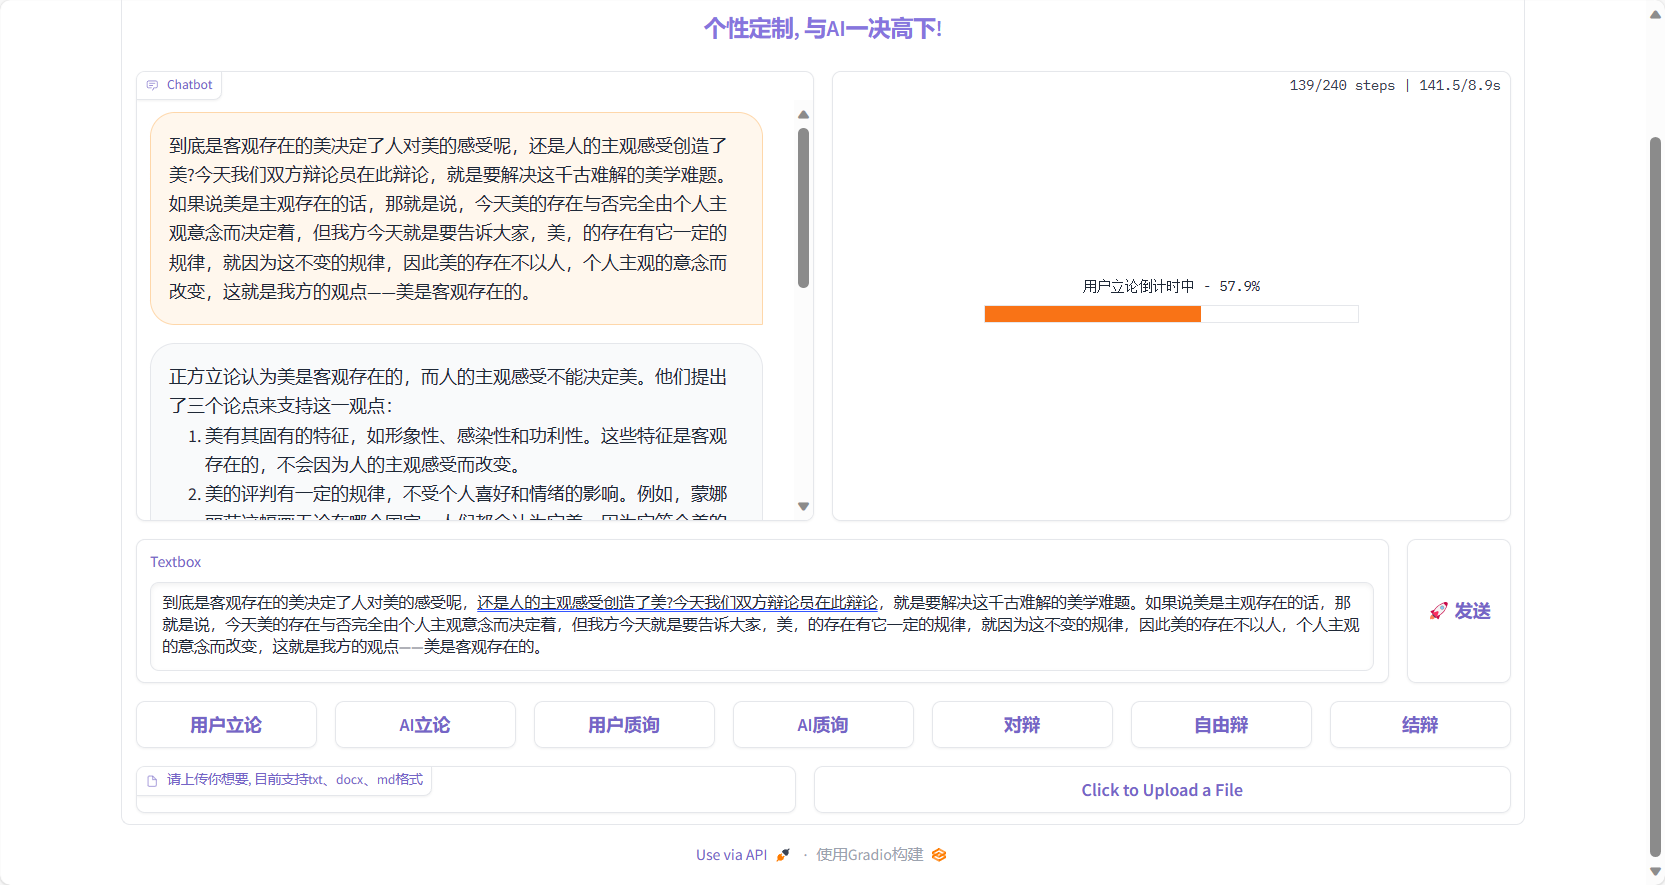
\includegraphics[width=0.8\textwidth,height=0.4\textwidth]{AI自定义实操.png}
        	\caption{自定关卡展示}
        \end{figure} 
        
         \subsection{AI辩手广场}
        \zw{在AI辩手广场部分,我们可以定制并发布独一无二的辩手到公共平台,大家也可以探索或者搜索我们的辩手并后续使用。在辩手生成部分,我们不仅提供常规的头像,描述,辩风等功能,还基于星火助手API实现了一个输入需求扩充完善辩风提示词的功能,从而帮助零基础小白生成强力辩手。}
        \begin{figure}[H]
        	\centering
        	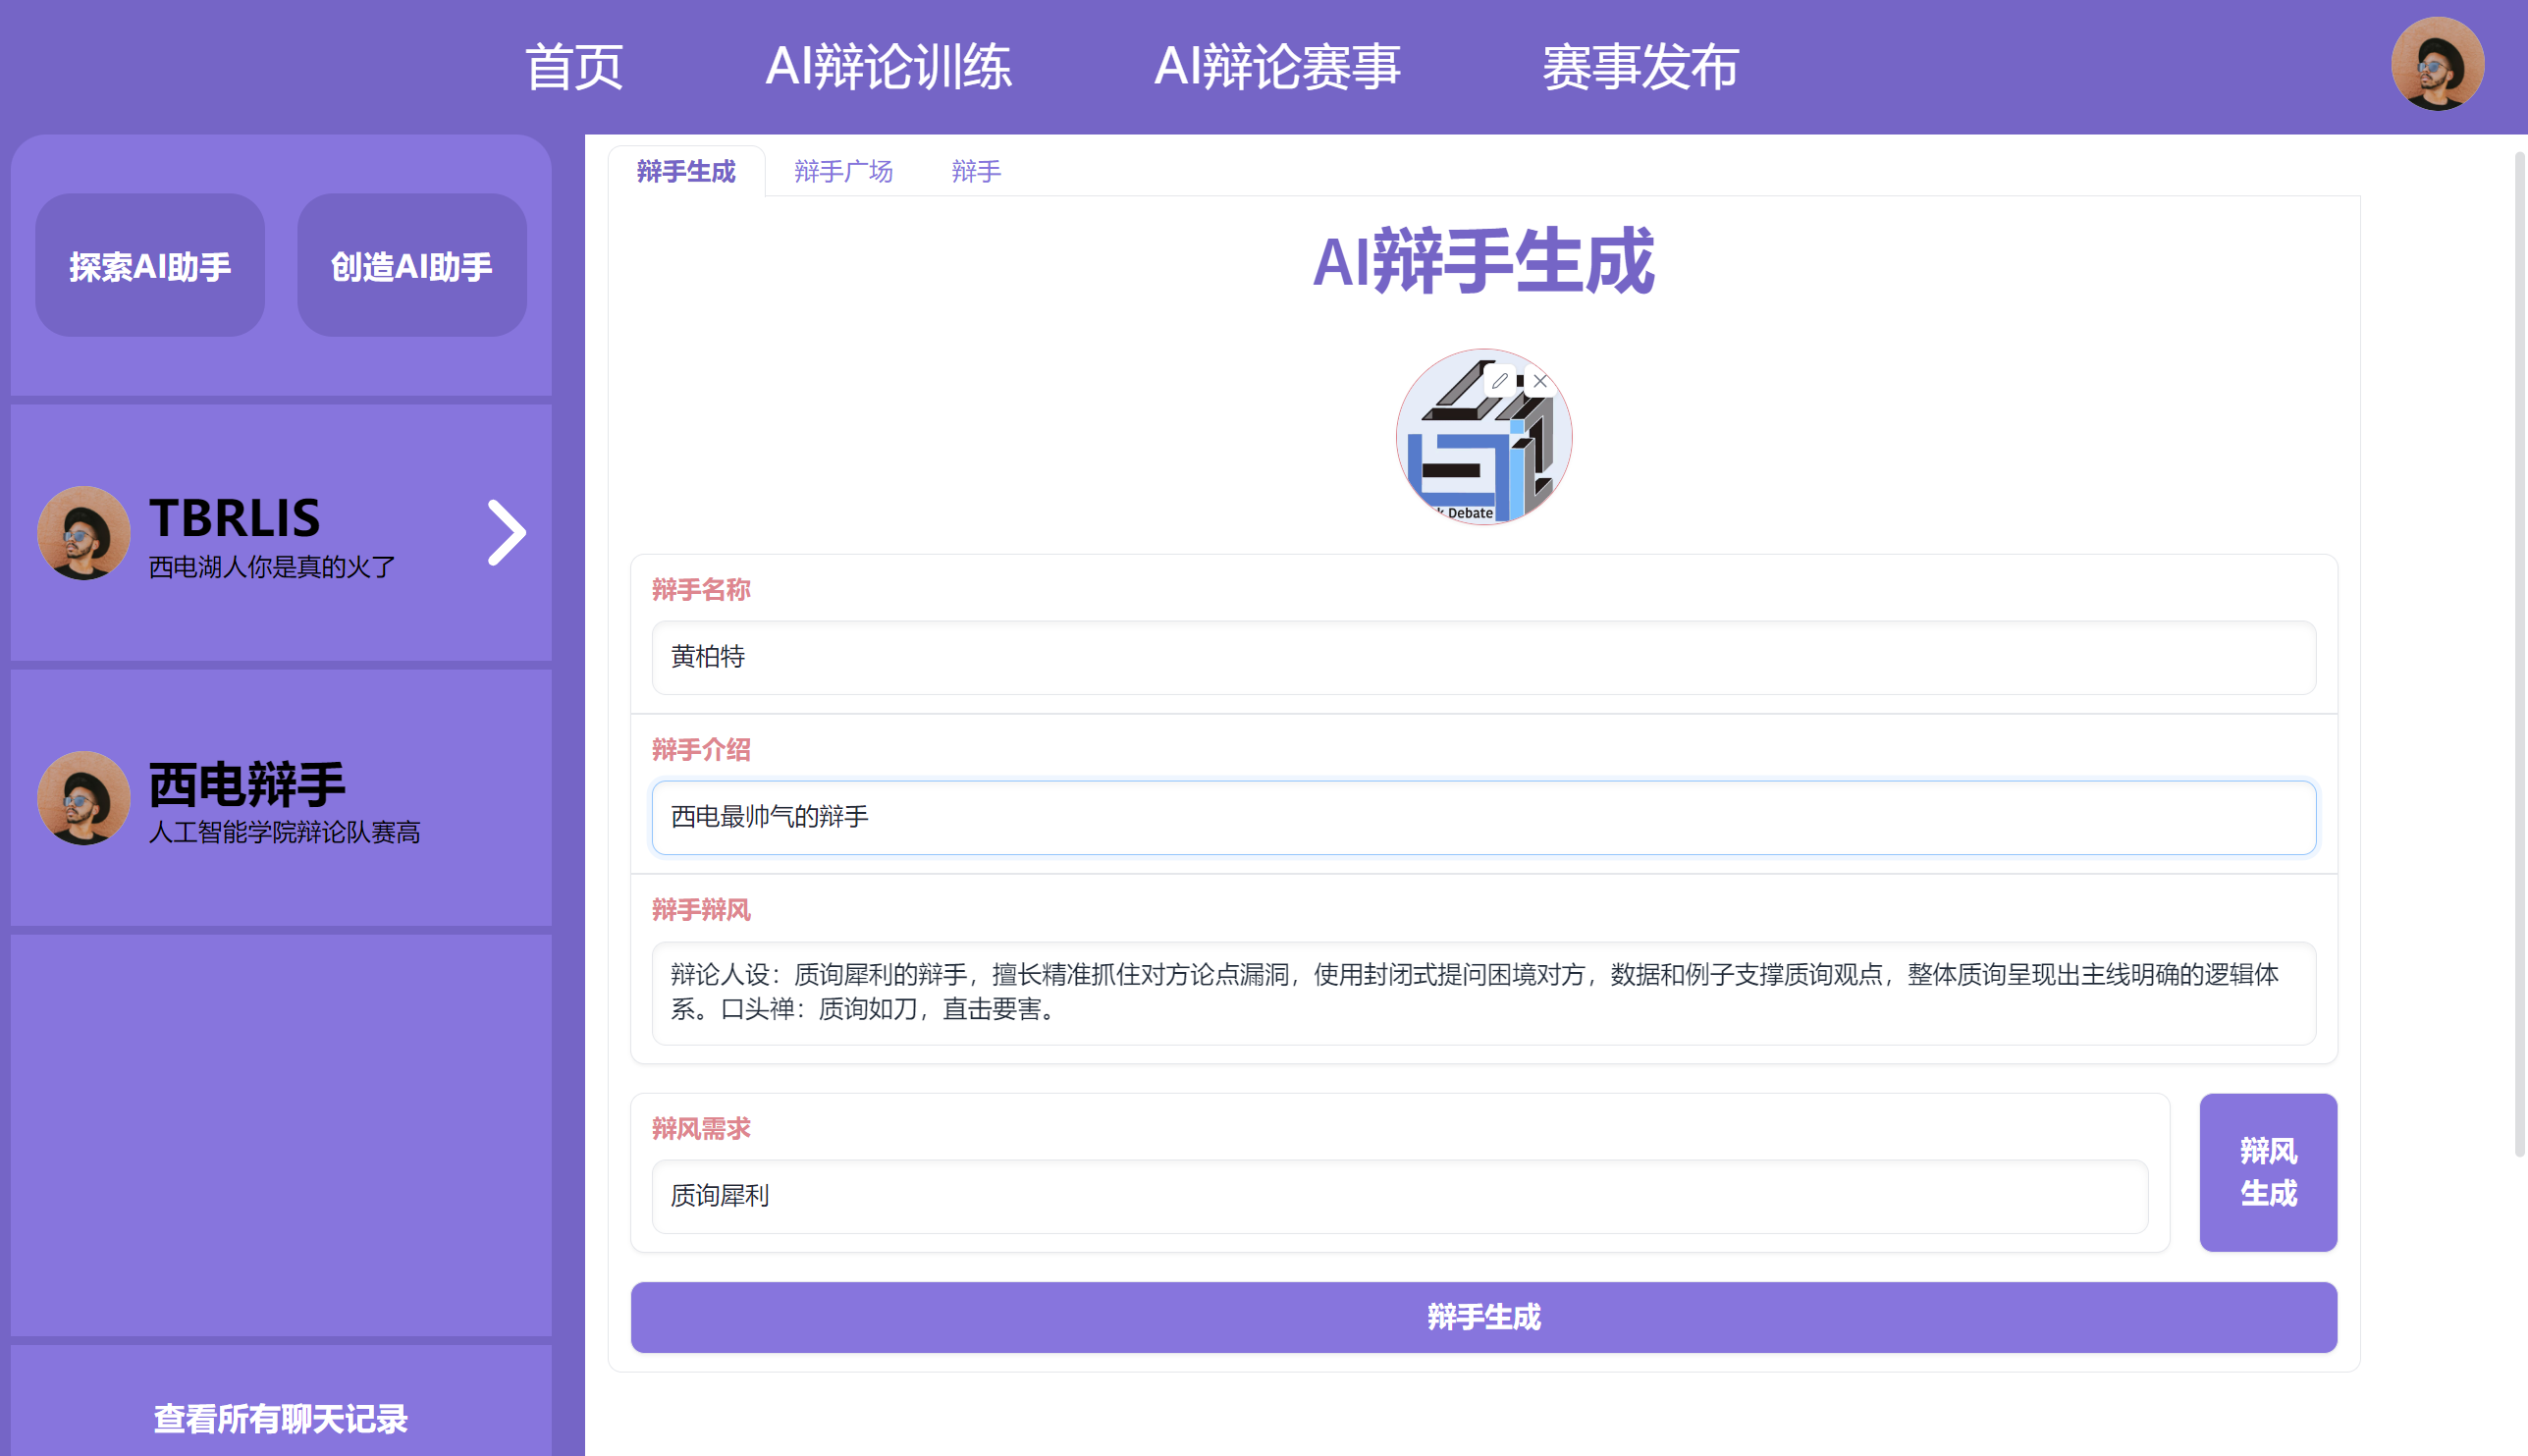
\includegraphics[width=0.8\textwidth,height=0.4\textwidth]{AI辩手生成.png}
        	\caption{AI辩手生成}
        \end{figure} 
        \zw{在AI辩手广场我们可以一键显示全部发布的AI辩手,也可以根据名称查询特定的AI辩手。}
        \begin{figure}[H]
        	\centering
        	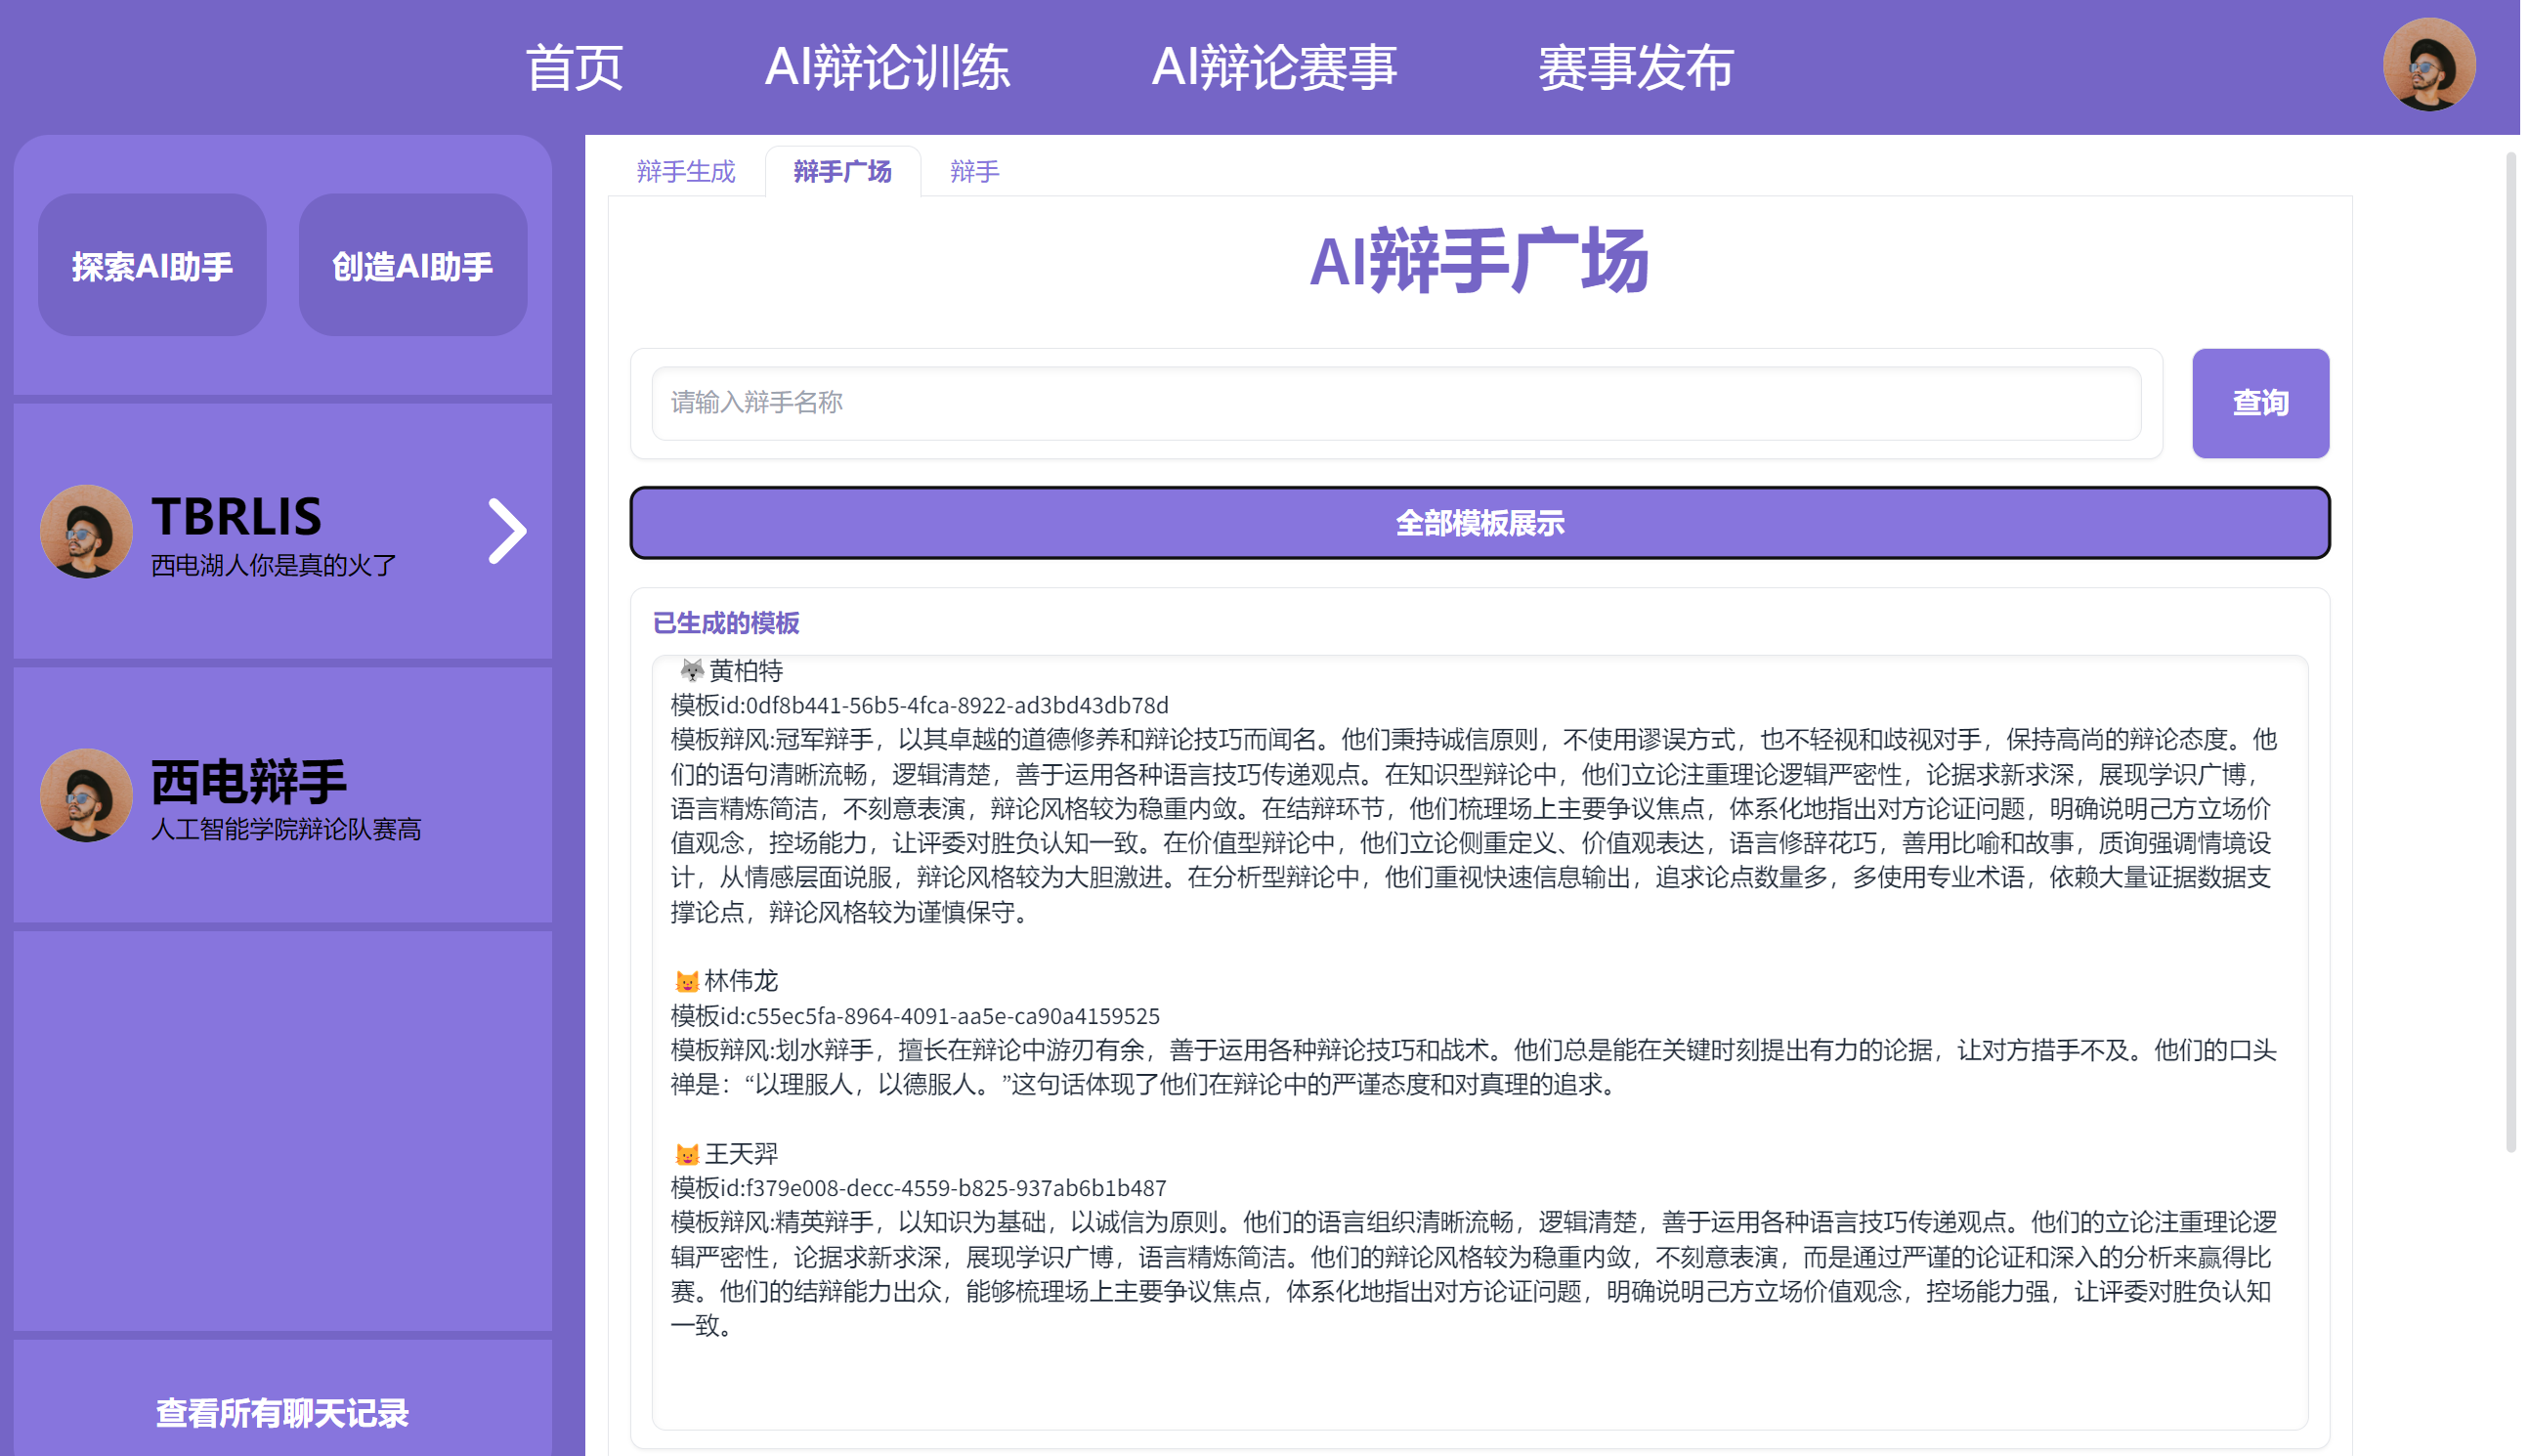
\includegraphics[width=0.8\textwidth,height=0.4\textwidth]{AI辩手广场.png}
        	\caption{全部AI辩手展示}
        \end{figure} 
         \begin{figure}[H]
        	\centering
        	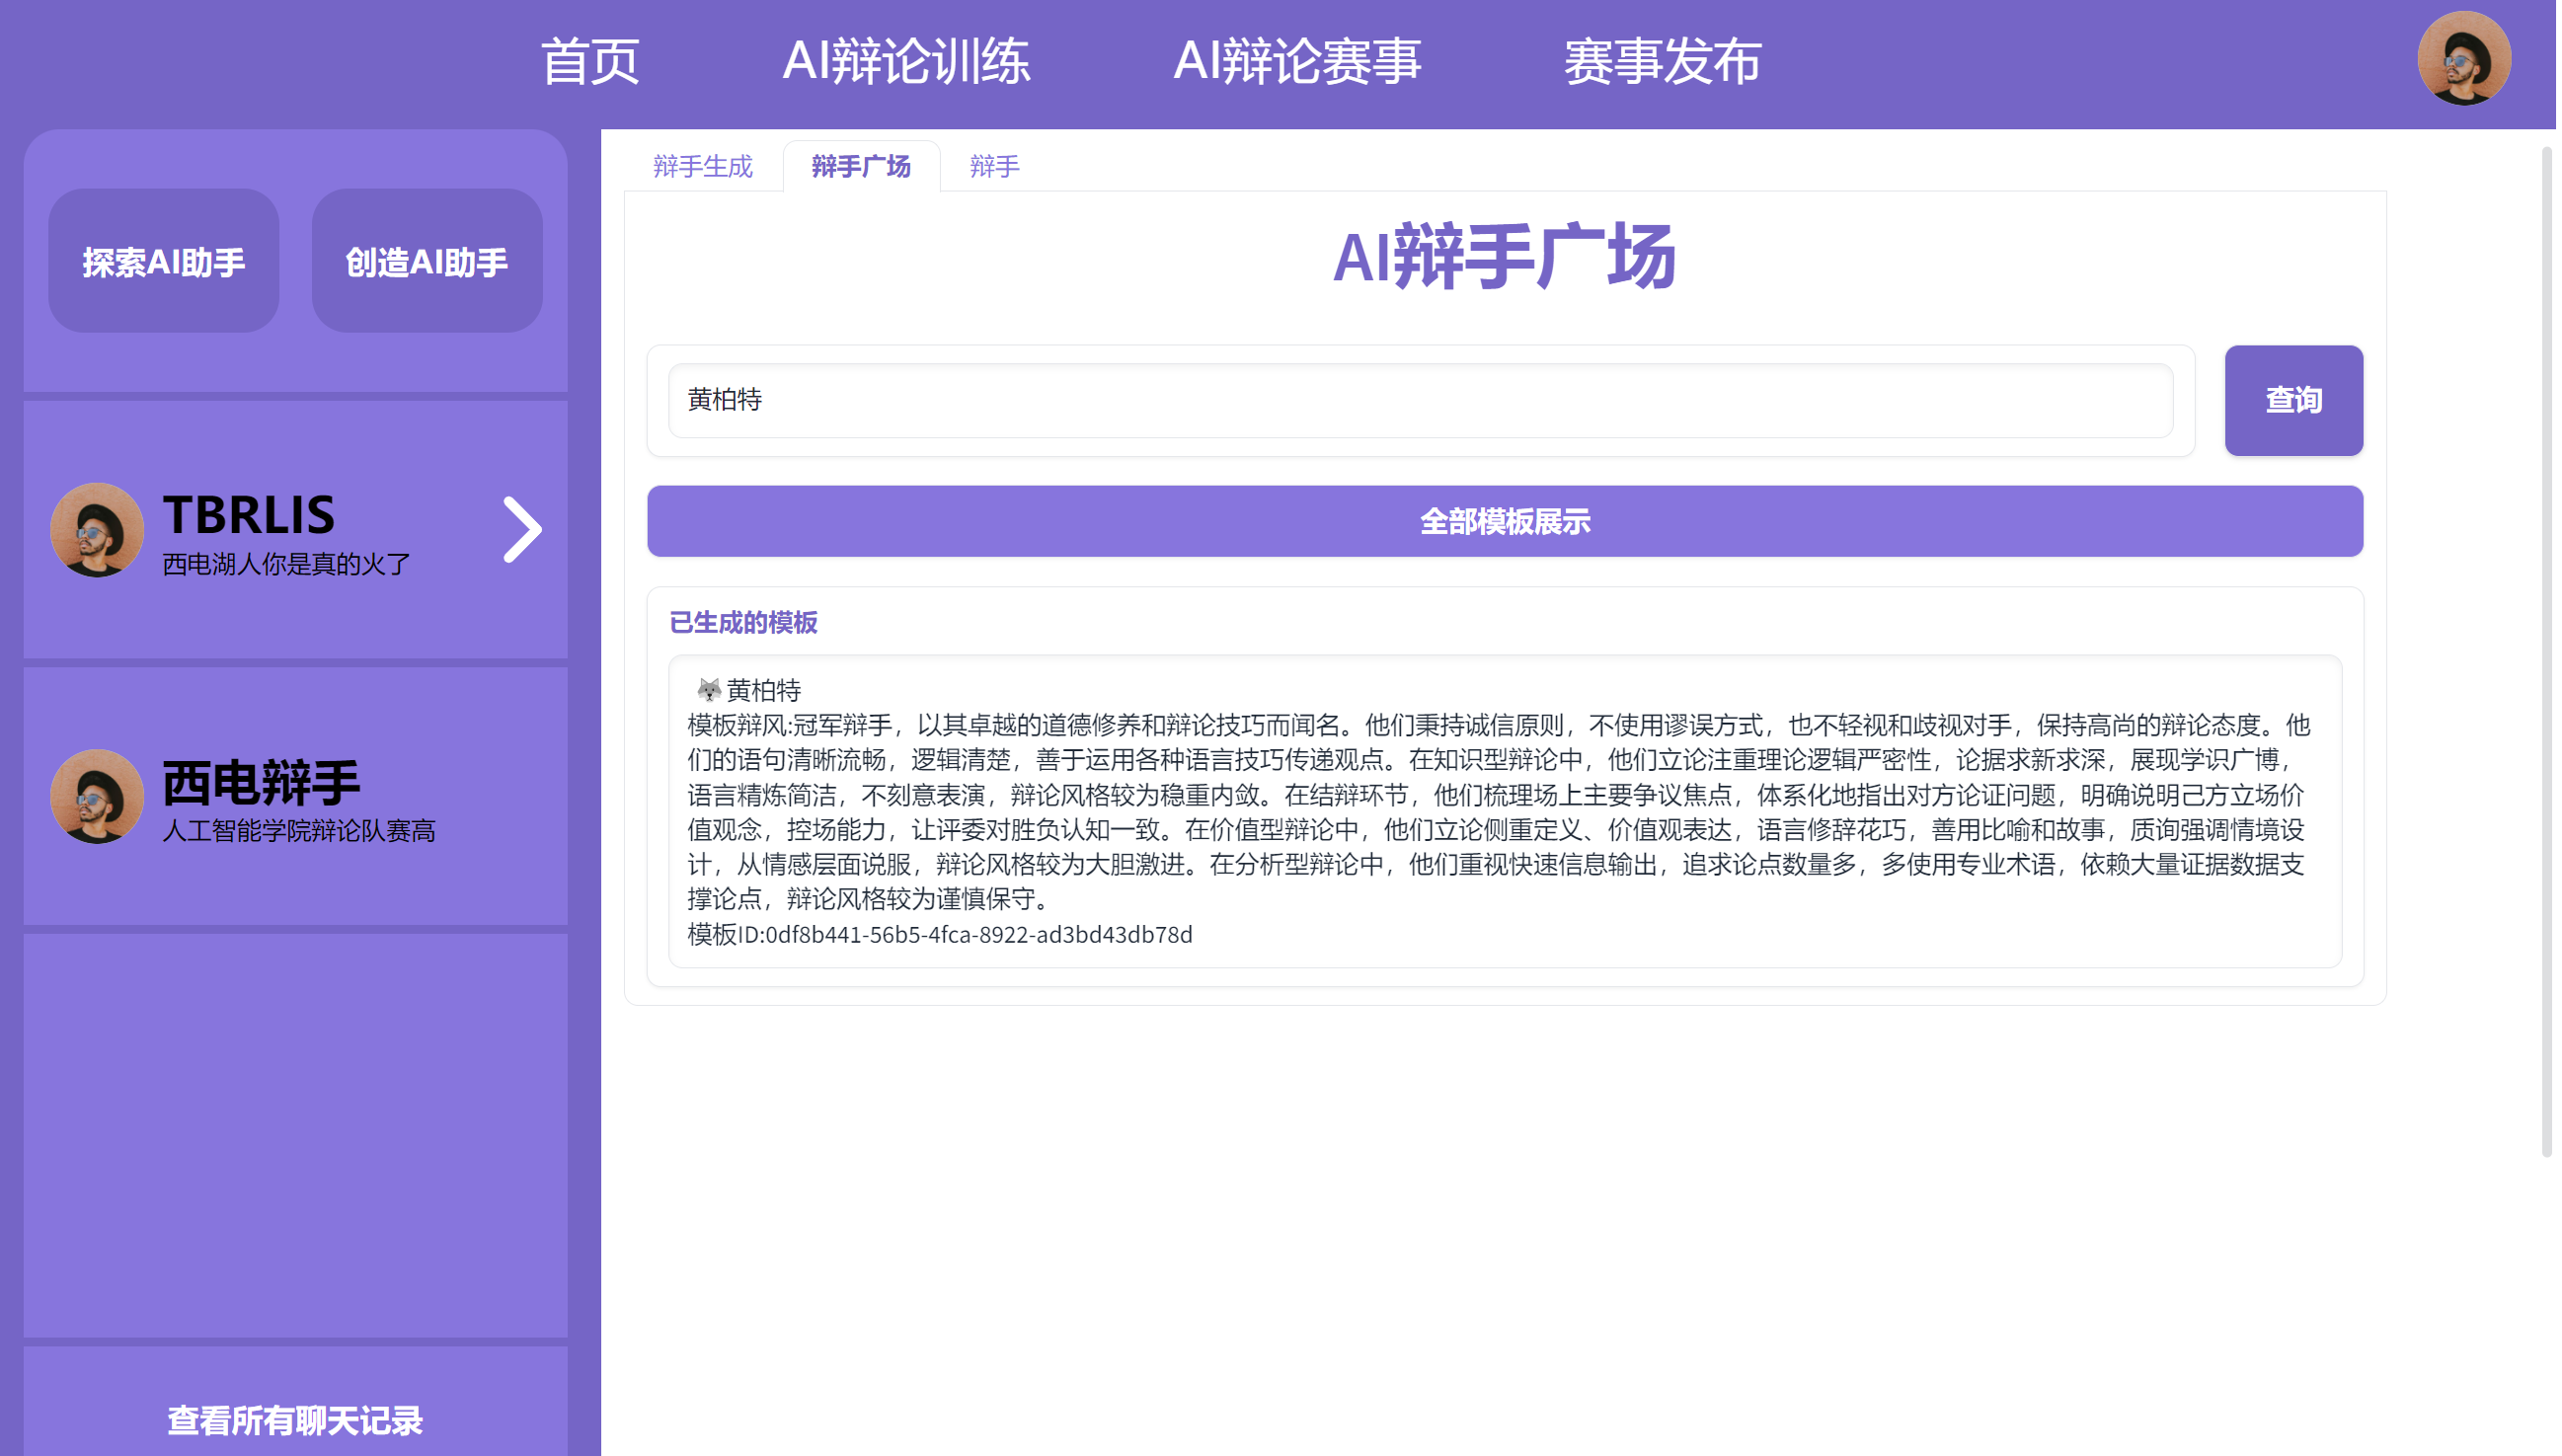
\includegraphics[width=0.8\textwidth,height=0.4\textwidth]{AI辩手查询.png}
        	\caption{指定AI辩手查询}
        \end{figure} 
        
        \subsection{聊天记录}
             \zw{我们还为每一次辩论,保留了聊天记录,助力辩手看到自己的成长过程。}
        \begin{figure}[H]
        	\centering
        	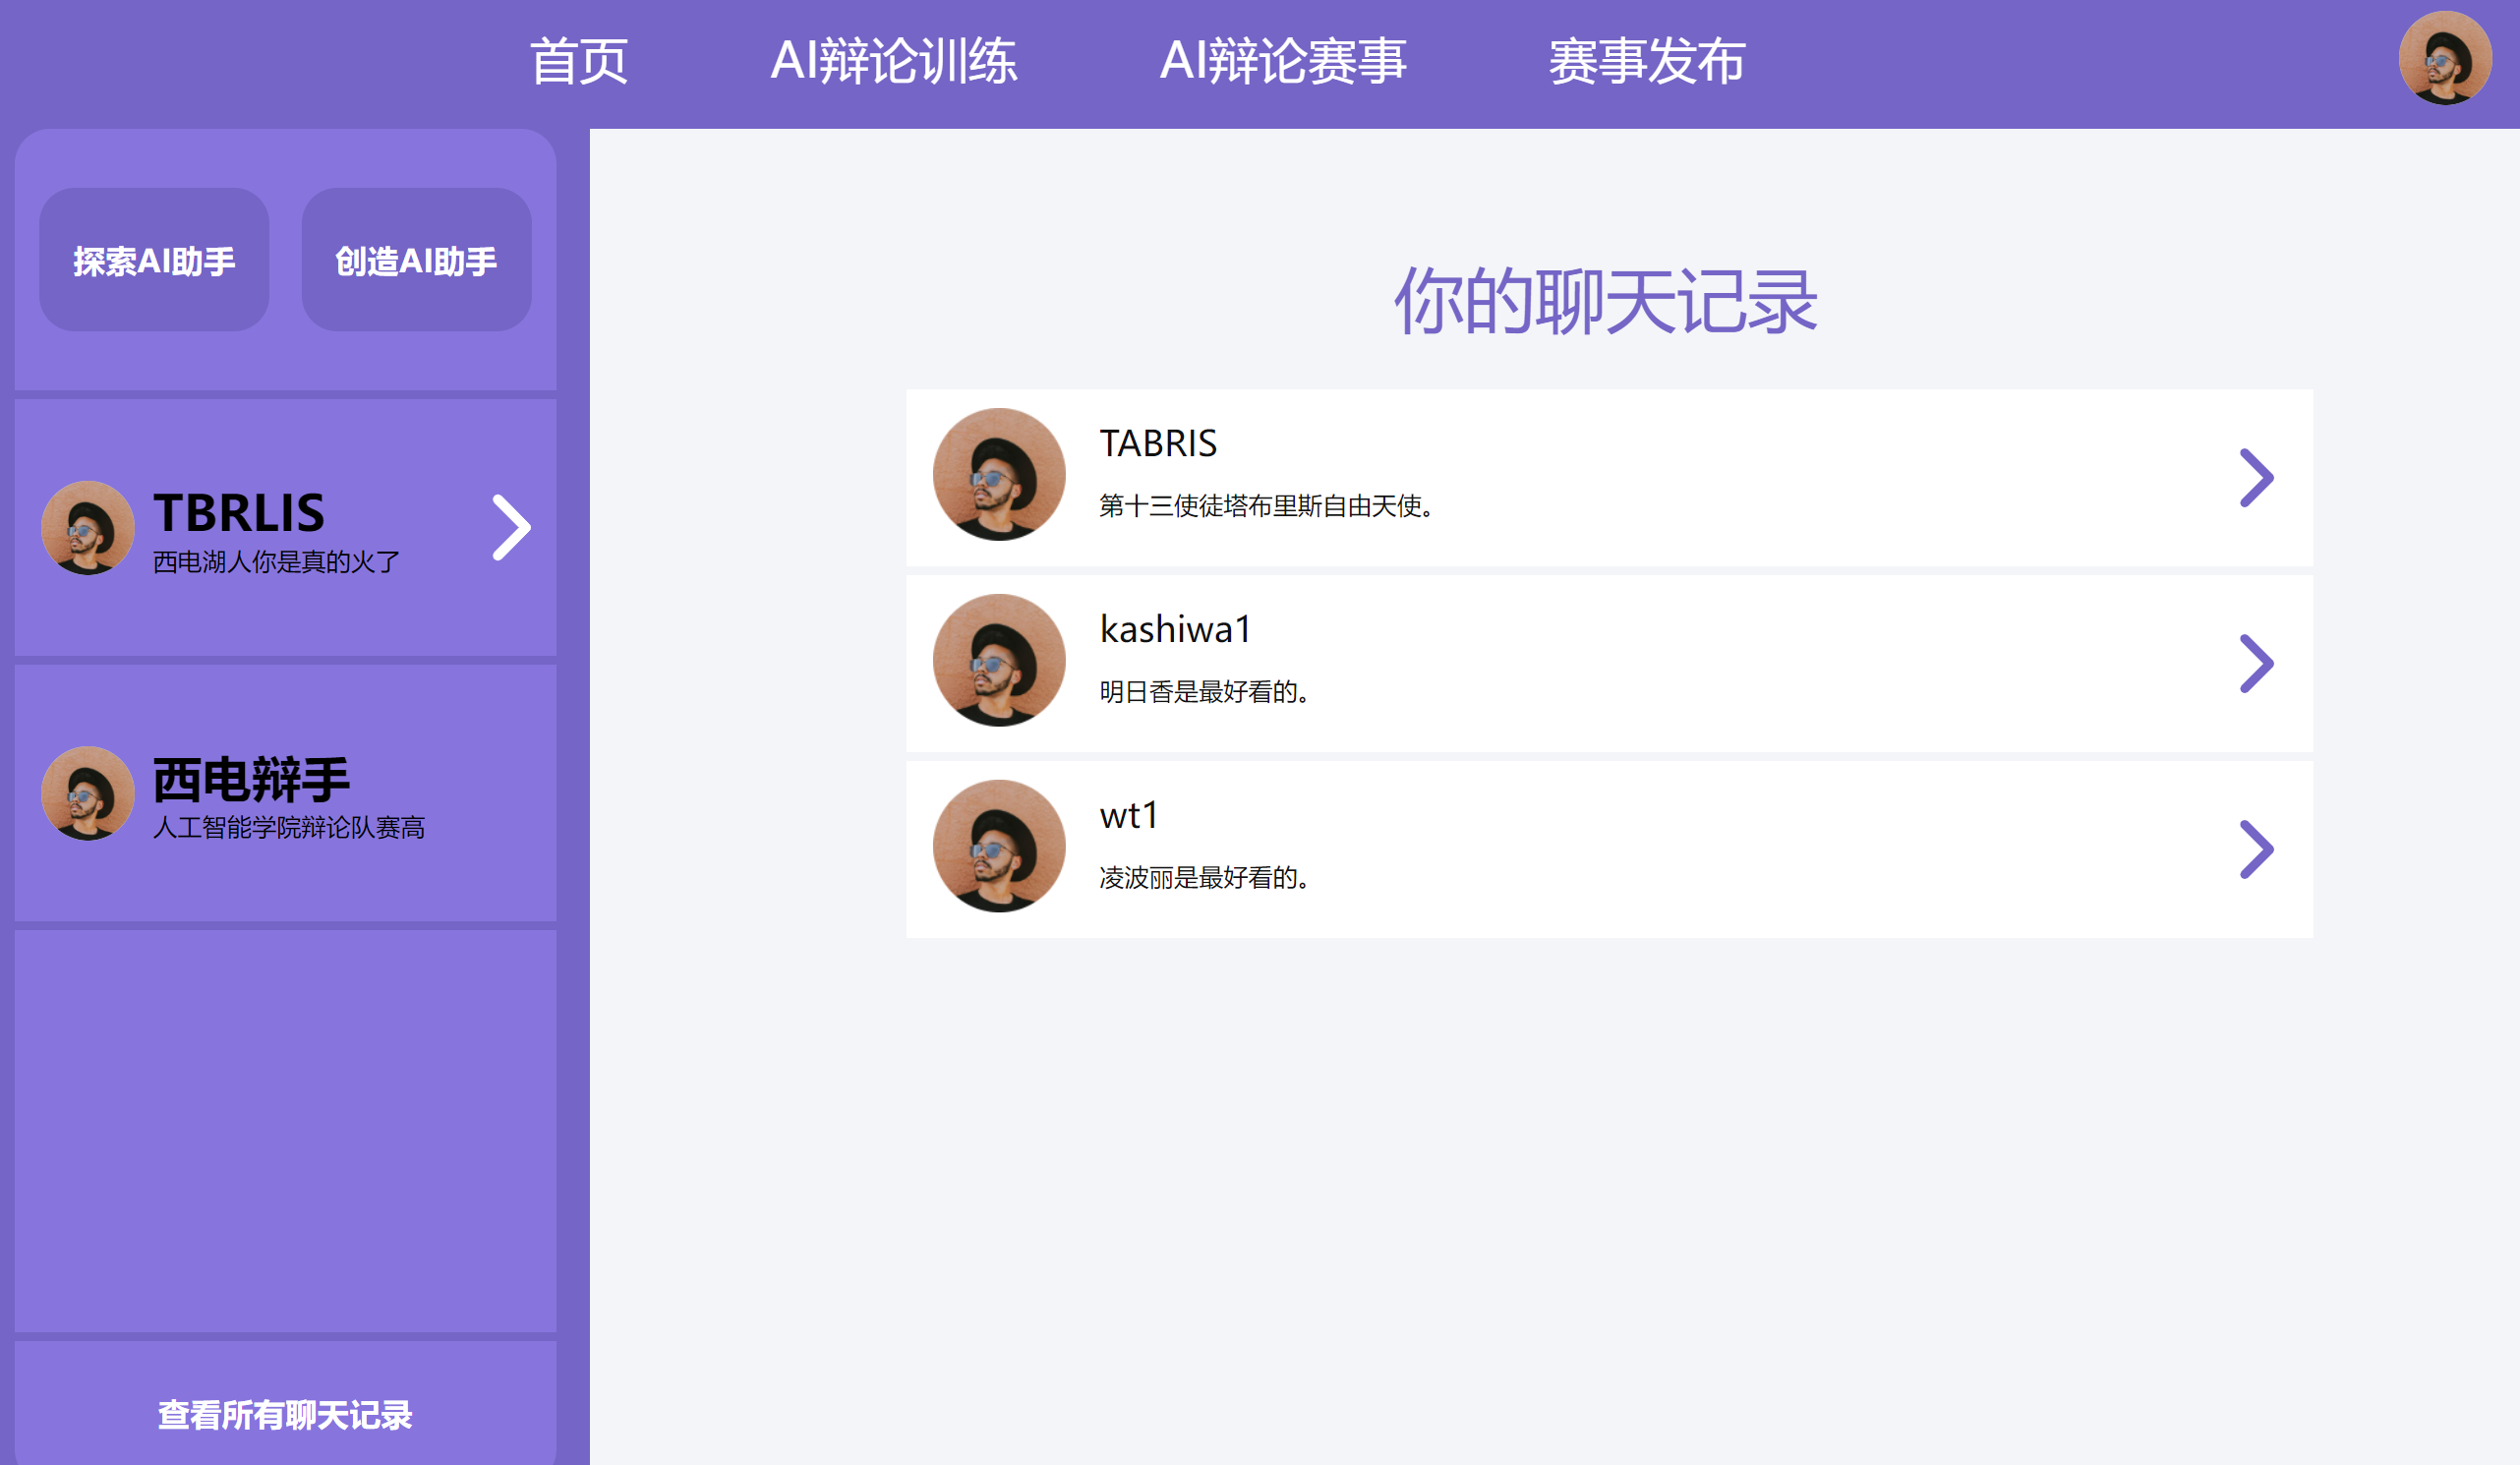
\includegraphics[width=0.8\textwidth,height=0.4\textwidth]{聊天记录.png}
        	\caption{聊天记录}
        \end{figure} 
        
         \subsection{赛事发布}
        \zw{我们还简单设计了赛事发布界面,后续赛事将围绕人人对战,人机对战,机机对战,人机团队混合对战等创新辩论模式建设成一个完整的辩论赛事平台。}
        \begin{figure}[H]
        	\centering
        	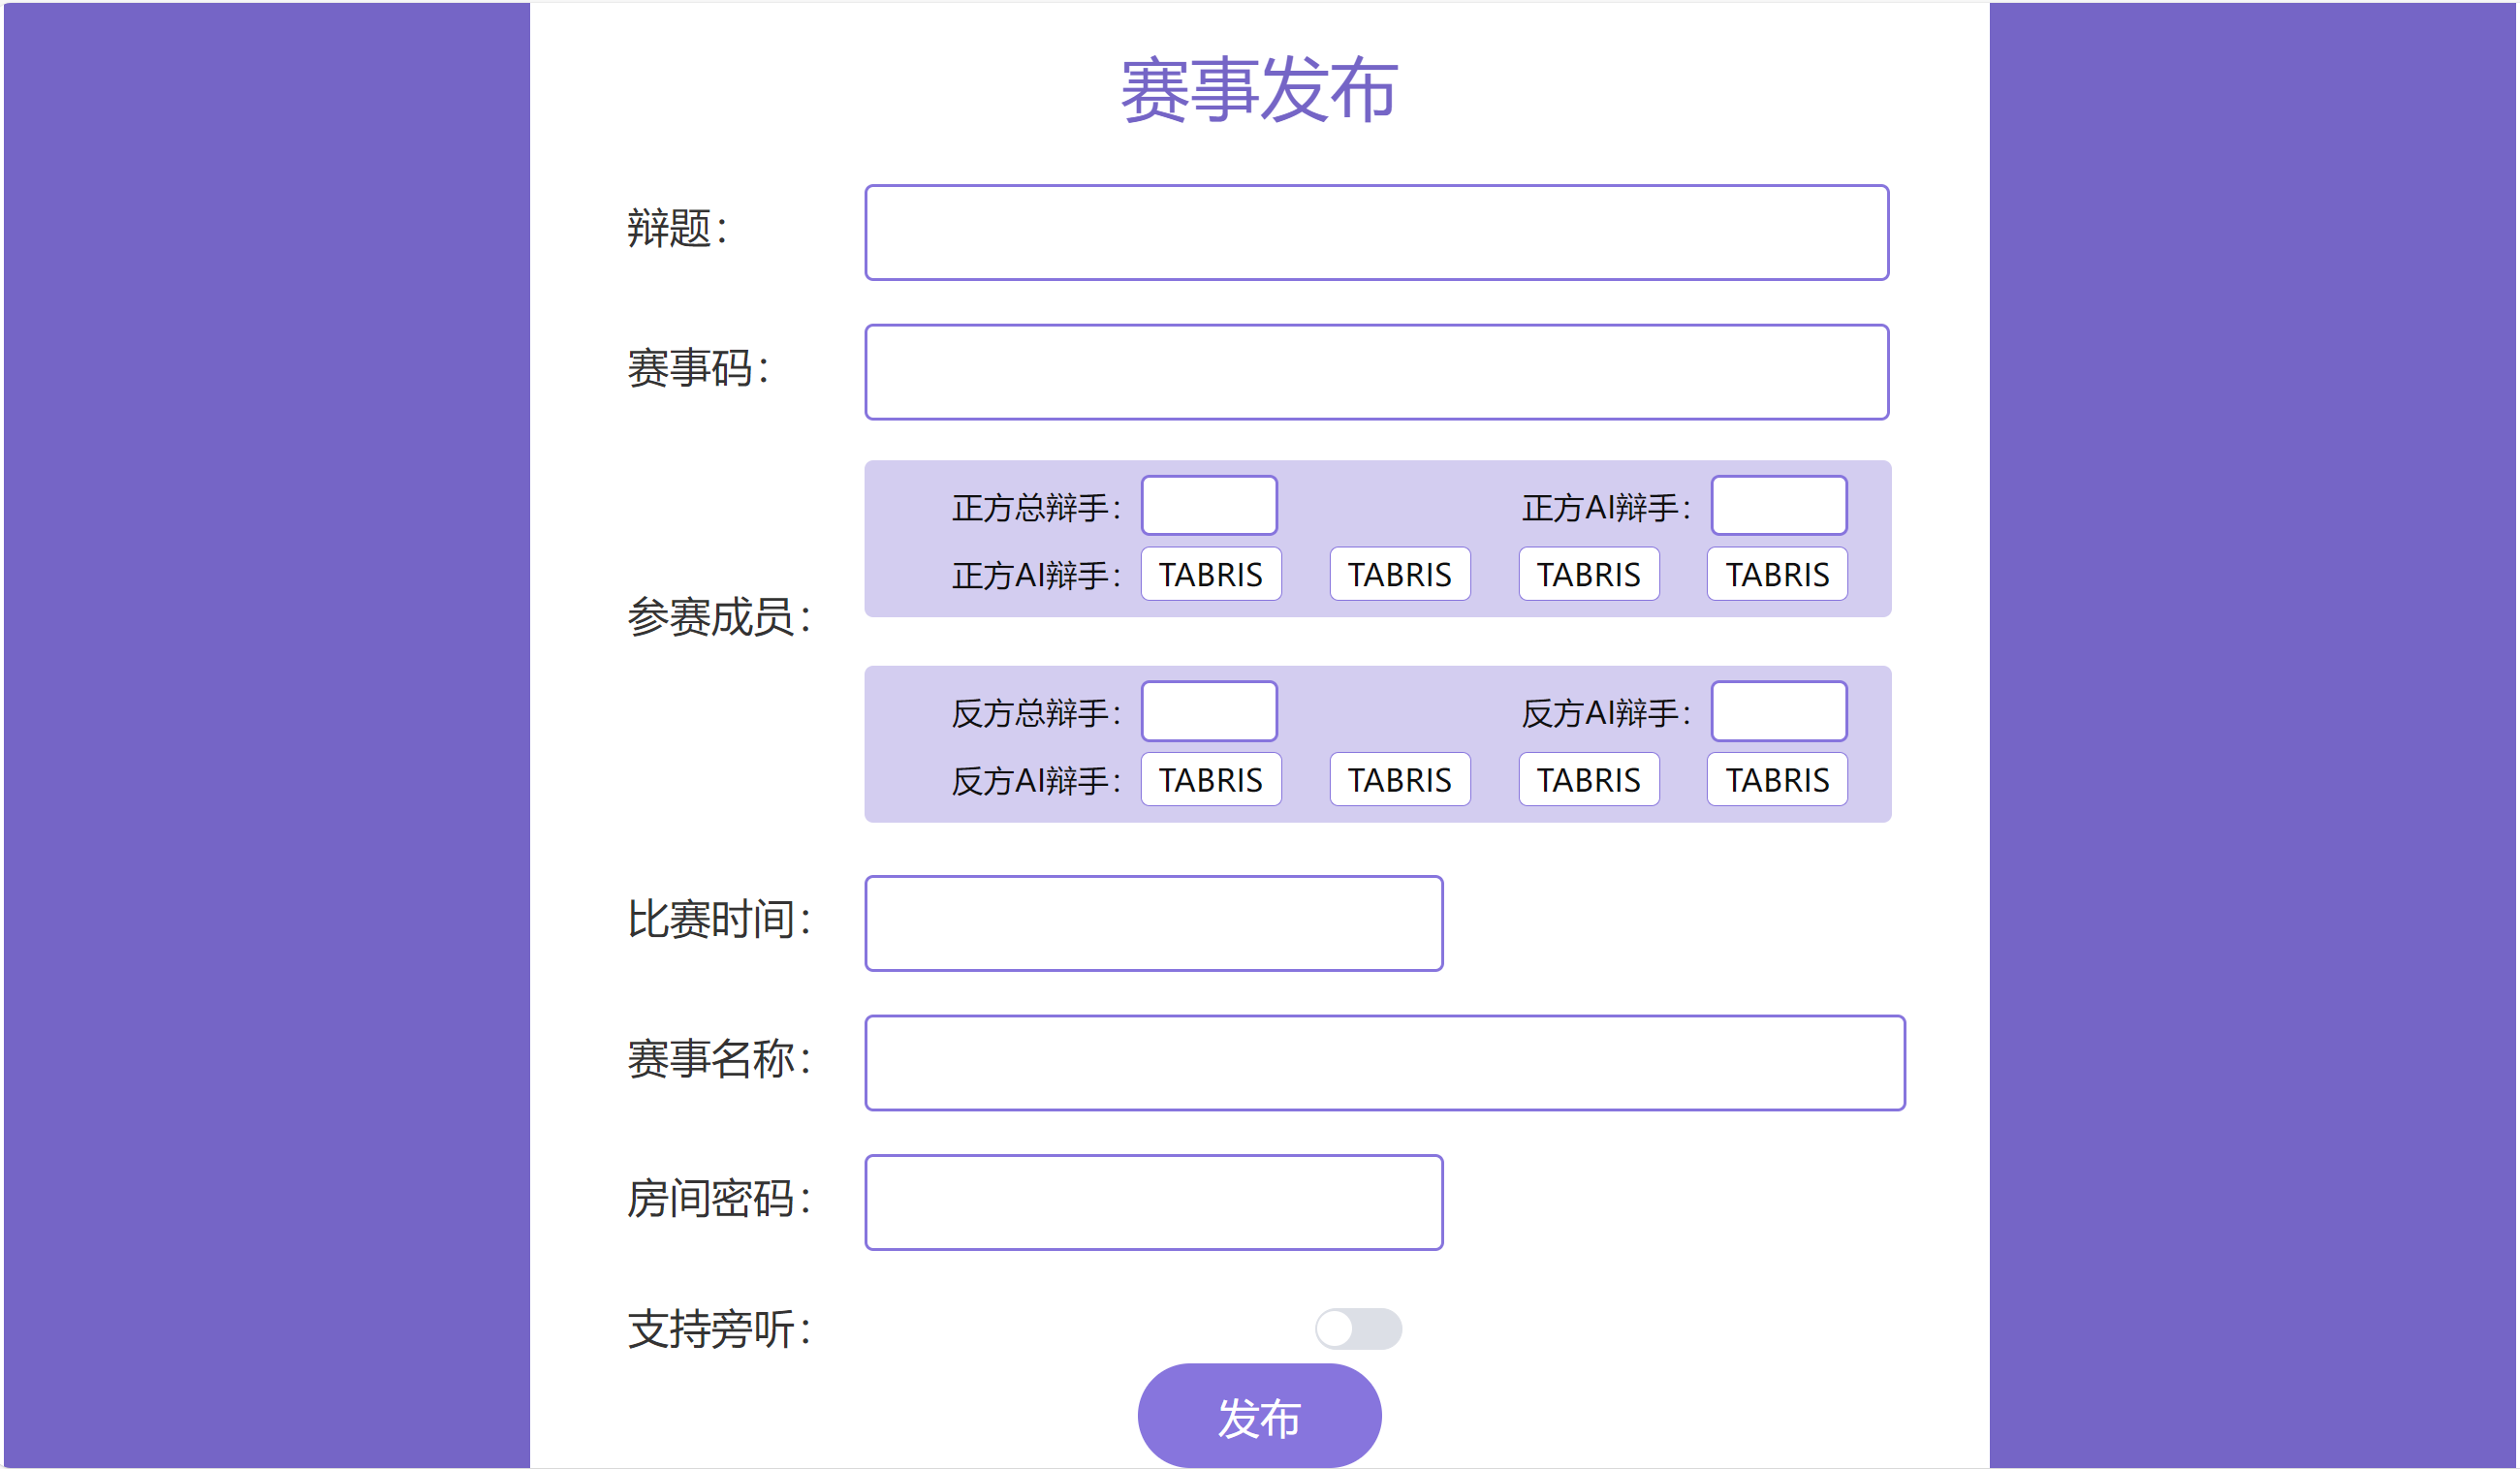
\includegraphics[width=0.8\textwidth,height=0.4\textwidth]{AI赛事发布.png}
        	\caption{赛事发布}
        \end{figure} 
        
        
        \section{拓展改进计划}
        \zw{由于时间资金与人员方面的诸多限制,我们的功能还有很多待完善之处,设想的产品需求也有很多没来得及实现,因此我们后续将围绕以下几点进行完善:}
        \item  \zw{1. 完善辩论赛事,实现智能辩手vs智能辩手,人vs智能辩手,人与智能辩手团队合作vs别的团队有趣辩论形式}
        \item  \zw{2. 完善知识库,让SparkDebate的专业性和内容丰富度更强大。}
        \item  \zw{3. 增设热点分析区块,挖掘并发布当下热点同时提出常见论点,革新当下的热点讨论模式并作为平台的流量入口}
        \item  \zw{4. 添加政策辩、法庭辩论等模式,让SparkDebate能够用于法律与政策的分析与决策支持。}
        \item  \zw{5. 推出app端,产品正式上线。}

		




	
\end{document}